%!TEX program = xelatex
\documentclass[a4paper,11pt,openany]{book} % twoside
\usepackage[]{geometry}
% \documentclass[twoside, 12pt]{article}

\usepackage{url}
\usepackage{fontspec}
\usepackage{lmodern}
\usepackage{csquotes}
\usepackage{graphicx}
\usepackage[rgb]{xcolor}
\graphicspath{ {img/} }
% \usepackage{polyglossia}
\usepackage{xunicode}
\usepackage{xltxtra}
\usepackage{todonotes}
\usepackage{epstopdf}
% \usepackage{fancyhdr}
\usepackage[czech]{babel}
\usepackage[pagestyles,medium]{titlesec}
\usepackage{setspace}
% \usepackage[sorting=nyt,style=apa]{biblatex}

\newcommand{\td}[2][]{
	{\todo[size=\footnotesize]{#2}}
}

\newcommand\exmp{\textsf}

\newpagestyle{sensible}{
	\headrule\sethead{}{}{\MakeUppercase{\chaptertitle}}
	\setfoot{}{\thepage}{}
}

% \renewcommand{\chaptermark}[1]{ \markboth{#1}{#1} }
% \renewcommand{\sectionmark}[1]{ \markright{#1}{} }

% \fancyhf{} % clear header and footer
% \fancyhead[R]{\rightmark} % section title on the left
% \fancyfoot[C]{\thepage}   % page number on the right

\setlength\emergencystretch{2em}
\setlength\headheight{14pt}
\setstretch{1.1}
\setcounter{secnumdepth}{4}

\widowpenalty10000
\clubpenalty10000

\hyphenation{выпа-дений}

% \setmainlanguage{czech}
\setmainfont[Ligatures=TeX]{CMU Serif Roman}

% \usepackage[english,czech]{babel} % main language of the document must be last
\usepackage[
   backend=biber
  ,style=iso-authoryear
  ,sortlocale=cs_CZ
  ,autocite=footnote
  ,maxnames=2
  ,minnames=1
  ,urldate=long
  ,spacecolon=true
  ]
  {biblatex}
% \usepackage[backend=biber, style=authoryear, sortlocale=cs_CZ, minnames=1, maxnames=2]{biblatex}

\addbibresource{bibliografie.bib}

\newcommand{\sign}[1]{%      
  \begin{tabular}[t]{@{}r@{}}
  \makebox[2.5in]{\dotfill}\\
  \strut#1\strut
  \end{tabular}%
}


\begin{document}
	\clearpage
	\pagenumbering{gobble}

	\begin{titlepage}
		\begin{center}
			{\Large\uppercase{Masarykova univerzita}}

			\vspace{1em}

			{\Large Filozofická fakulta}

			\vspace{1em}

			{\large Ústav českého jazyka}

			\vspace{1em}

			{\large Český jazyk se specializací počítačová lingvistika}

			\vspace{11em}

			{\large David Klement}
			
			\vspace{3em}
			
			{\LARGE\bf Grafické rozhraní pro prediktivní zápis textu}

			\vspace{1.5em}

			{\Large Bakalářská diplomová práce}

			\vfill
			\vspace{3em}
			Vedoucí práce: RNDr. Adam Rambousek, Ph.D.
			
			2015
		\end{center}
	\end{titlepage}


% \pretolerance=1000
	
\par
\par\vspace*{\fill}
	\pagestyle{plain}
\pagenumbering{roman}
\begin{flushright}
	Prohlašuji, že jsem bakalářskou diplomovou práci vypracoval samostatně s~využitím uvedených pramenů a~literatury.

	\vspace{3em}

	    \makebox[2.5in][r]{\dotfill}
	    
	    autor práce

	    \par

\end{flushright}
\clearpage

\par
\par\vspace*{\fill}

Na tomto místě bych rád poděkoval Adamu Rambouskovi za veškerou pomoc, trpělivost a~všechny odborné rady, jež mi ochotně poskytoval po celou dobu psaní této práce. 

Děkuji také své rodině za morální podporu, Janu Šedovi za cenné rady v~oblasti programování v~JavaScriptu a~Marii Staré za pomoc s~jazykovými korekturami.

\clearpage

\section*{Abstrakt}

Tato bakalářská práce shrnuje vývoj systémů pro predikci textu, porovnává je a~popisuje technologie, na nichž jsou tyto systémy postaveny. Dále se zabývá hodnocením účinnosti vybraných metod zadávání textu a možnostmi jejího zlepšení použitím různých prediktivních systémů. Praktická část práce je zaměřena na vývoj grafického uživatelského rozhraní pro prediktivní zápis textu, které je vhodné pro zařízení bez dotykové obrazovky a~s klasickou klávesnicí QWERTY. Toto rozhraní zobrazuje predikce generované serverovou částí aplikace, která využívá jazykový model ve formě n-gramů vytvořených z~největšího českého korpusu czTenTen.

\section*{Abstract}

This bachelor thesis summarizes development of text prediction systems, compares these and describes technologies these systems are built upon. Furthermore, the thesis outlines methods of evaluation for selected text input systems as well as text prediction systems. The part about implementation is focused on the development of the graphical user interface for predictive text entry that is well suited for devices without a~touchscreen and with a~benefit of a~full QWERTY keyboard. This user interface presents a~user with predictions produced by the server-side application which uses n-grams generated from the largest Czech corpus, czTenTen, as a~language model.

\section*{Klíčová slova}

predikce textu, jazykový model, zadávání textu, KSPC

\section*{Keywords}

text prediction, language model, text input, KSPC

\clearpage

\tableofcontents

\clearpage

\newgeometry{top=2cm}

\chapter*{Úvod}\label{uvod}

\addcontentsline{toc}{chapter}{Úvod}

\pagenumbering{arabic}

Různé implementace predikce textu se objevují v~mobilních telefonech a~elektronických osobních asistentech již přes dvě dekády, přičemž jejich hlavním úkolem je usnadnit zadávání textu na klávesnicích mobilních zařízení. V~poslední době se s~rozmachem chytrých telefonů objevily systémy predikce textu (a automatické opravy slov, která s~ní souvisí) i~pro jednoznačné klávesnice typu QWERTY, a~to z~důvodu zvýšení komfortu psaní. Tyto systémy mají obvykle dvě nevýhody. První z~nich je závislost na konkrétním operačním systému, konkrétním zařízení (především v~případě starších telefonů) či na konkrétní aplikaci, která zajišťuje zobrazení klávesnice na dotykovém displeji. Takové systémy tudíž nejsou použitelné například pro psaní na stolním počítači na klasické klávesnici QWERTY. Druhou nevýhodou je fakt, že systémy většinou musí spoléhat pouze na lokálně uložená jazyková data, která tak musí být relativně kompaktní co do datové velikosti a~nemusí tedy obsahovat takové množství dat, aby uživatel nebyl omezován nedokonalostmi jazykového modelu.

Protipólem velkého množství aplikací pro predikci textu pro mobilní zařízení je téměř prázdná množina takových aplikací pro klasické počítače se standardní klávesnicí QWERTY. Textové procesory typu LibreOffice Writer\footnote{\url{https://www.libreoffice.org/discover/writer/}} mívají vestavěné primitivní způsoby doplňování, které ale čerpají data pouze z~textu, který je v~danou chvíli v~editovaném dokumentu. Textové editory typu Atom\footnote{\url{https://atom.io/}} mívají podobnou funkcionalitu, navíc například při editaci programového kódu nabízí relativně komplexní doplňování, ale pouze podle předem připravených šablon.

Cílem této práce je tedy vytvořit implementaci systému predikce textu, která bude čerpat data z~velkého korpusu textů, a~navíc bude nezávislá na platformě. Vzhledem k~tomu, že korpusová data není možné uchovávat na straně klienta, bylo logickým krokem zvolit model klienta a~serveru, který bude zajišťovat generování predikcí. Tento systém na serveru již v~době tvorby této práce existoval, což umožnilo soustředit se především na vývoj uživatelského prostředí. 

Pro zajištění co nejvyšší kompatibility s~různými systémy byla zvolena forma zásuvného modulu do CKEditoru\footnote{\url{http://ckeditor.com/}}, webového editoru HTML (Hyper Text Markup Language). Použitými technologiemi tedy byl především JavaScript pro programovou logiku, Ajax (asynchronous JavaScript and XML (Extensible Markup Language)) pro komunikaci se serverem a~HTML a~CSS (Cascading Style Sheets) pro uživatelské rozhraní.

\restoregeometry

\part{Teoretická část}
\pagestyle{sensible}

\chapter{Obecně o~predikci textu}

\section{Definice pojmu predikce textu}

Predikce textu, neboli automatické doplňování textu (angl. autocomplete) je funkce v~aplikaci, která na základě uživatelského vstupu (většinou prvních několika znaků slova) doplňuje zbytek části textu (většinou slova). V~ideálním případě funkce jednoznačně rozpozná, co chtěl uživatel napsat, a~nabídne mu právě to doplnění, jež uživatel chce. V~praxi obvykle uživatel dostává na výběr z~několika možností, které systém vyhodnotil jako nejpravděpodobnější doplnění vstupu. Systémy se liší způsobem zužování výběru možností a~jejich řazením, stejně jako vizuálním podáním nabídky.

Systémy automatického doplňování textu obecně fungují nejlépe v~implementacích na omezených doménách, tzn.~například doplňování e-mailových adres v~e-mailových klientech, klíčových slov určitého programovacího jazyka v~programátorských editorech či doplňování ve formulářových polích s~předem vymezeným očekávaným vstupem. 

\section{Disambiguace, automatické opravy a~predikce textu}

Automatické opravy a~predikce textu jsou dva velmi úzce svázané pojmy. Prvním se myslí opravení textu poté, co jej uživatel chybně zadal, druhým pak nabídnutí textu uživateli předtím, než jej zadal. Na pomezí těchto dvou technik se ještě vyskytuje třetí, a~to disambiguace vstupu z~nejednoznačné klávesnice. Všechny tyto tři techniky jsou úzce spjaty proto, že je nutné nejdříve nějakým způsobem odhadnout, co uživatel chtěl, případně bude chtít, napsat.

Ačkoliv je praktická část této práce zaměřena na predikci textu a~disambiguací se nezabývá, zdálo se vhodné popsat i~vývoj a~některé způsoby řešení problematiky disambiguace vstupu, protože řeší podobné problémy.

\section{Úskalí jazyků s~rozvinutou flexí}

Systémy pro predikci textu určené k~tvorbě volného textu jsou obvykle, jak bude zřejmé z~dalšího popisu jednotlivých aplikací, založeny na více či méně rozsáhlém lokálně uloženém slovníku jednotlivých slov či slovních spojení, ze kterého vybírají možná doplnění. Tyto systémy zpravidla umožňují uživateli přidávat manuálně slova, která napsal a~nejsou ve slovníku, což slouží jako základní uživatelské přizpůsobení. Lokální slovník má ovšem tu nevýhodu, že jeho velikost je značně limitována možnostmi zařízení, tj.~jeho paměťovou a~výpočetní kapacitou. To je problém především pro jazyky s~rozvinutou flexí, jako je čeština, které potřebují na rozdíl od analytických jazyků, např. angličtiny, poněkud větší množství tvarů jednotlivých slov. 

Rozdílnost angličtiny a~češtiny v~ohledu množství slovních tvarů připadajících na jedno lemma\footnote{základní slovní tvar} lze porovnat například na dvou velkých korpusech, enTenTen13 a~czTenTen12 \parencite{suchomel2012}. Jde o~korpusy vytvořené z~textů získaných na Internetu, které byly vyčištěny a~zbaveny duplikátů nástrojem Onion\footnote{\url{http://corpus.tools/wiki/Onion}}. Anglický korpus enTenTen13 obsahuje 39~452~714 slov a~37~366~565 lemmat \parencite{czTenTen12_info}. Naproti tomu český korpus czTenTen12 obsahuje slov 18~725~879 a~lemmat pouze 13~976~481 \parencite{enTenTen13_info}. V~češtině tedy podle výše uvedených dat připadá na jedno lemma 1,339 slovního tvaru, naproti tomu v~angličtině na jedno lemma připadá pouze 1,056 slovního tvaru. Je tedy vidět, že slovník pro češtinu by v~ideálním případě měl být minimálně 1,27× větší než slovník o~stejném množství lemmat pro angličtinu. Zde je na místě uvést, že to je ve srovnání s~údaji, jež uvádí \textcite{nemeth2012word}, velice málo. Ti totiž píší, že pro udržení míry chybovosti v~rozpoznávání řeči je pro němčinu potřeba slovník zhruba 4× větší a~pro maďarštinu dokonce 20× větší než pro angličtinu.

Vezmou-li se v~potaz teoretická data, vychází poměr slovních tvarů na lemma i~pro češtinu výrazně vyšší. Pro účely této práce byla provedena empirická analýza cca 500~nejčastějších slov v~češtině pomocí morfologického analyzátoru Majka. Tento experiment ukázal, že čeština je v~teoretickém poměru (unikátních) slovních tvarů na lemma skutečně relativně blízko maďarštině s~poměrem 17,537. Nutno podotknout, že se jedná o~tvary vzniklé nejen skloňováním a~časováním, ale i~záporkou {\it ne-}, stupňováním adjektiv či jejich kombinacemi.

% Problem: http://perso.telecom-paristech.fr/~chollet/Biblio/Congres/Audio/Eurospeech01/CDROM/papers/page2035.pdf pise, ze rozdil mezi eng a~hu je 20x, coz uplne nesedi k~te cestine tady z~korpusu, prodiskutovat s~christofem 

Množství slovních tvarů na lemma ve flektivních jazycích komplikuje implementaci slovníkových jazykových modelů do aplikací pro predikci textů v~těchto jazycích, protože je nutno uchovávat větší množství slovních tvarů než pro angličtinu. Stejně tak je žádoucí zohledňovat kontext, aby byly slovní tvary vybírány správně, protože například bez zohlednění syntaxe mohou predikce vést k~negramatickým větám. \parencite[5234--5235]{ghayoomi2009overview}

\chapter{Klíčové vlastnosti systému pro predikci textu}

Navzdory velmi odlišným způsobům použití systémů pro doplňování textů jsou některé jejich klíčové vlastnosti pro většinu implementací společné. Studie, které zkoumaly efektivitu těchto systémů, obecně docházejí k podobným závěrům, co se požadavků na tyto systémy týče. Ať jde o~vyhledávač typu Google\footnote{\url{https://www.google.com}} nebo o~predikci volného textu v~textovém editoru, musí systém mít několik vlastností, aby měl uživatel při užívání aplikace pocit, že mu doplňování textu skutečně pomáhá.  Primární je rychlost, s~níž aplikace možná doplnění uživateli zobrazuje. \textcite{nandi2007assisted} uvádí, že by odezva neměla převyšovat 100 ms. Tento faktor je rozhodující pro to, zda se uživatel rozhodne nabídnutá doplnění použít, nebo raději napíše zbytek textu sám. V~případě implementace predikce textu do editoru, kde uživatel zadává volný text, jímž si je relativně jist, je tato vlastnost pro uživatelovo rozhodnutí patrně klíčová. Naproti tomu ve vyhledávání lze očekávat, že uživatel bude ochoten počkat delší chvíli na zobrazení doplnění. S~tímto souvisí i~další vlastnost -- umožnit uživateli pohodlně nabízené predikce ignorovat \parencite{ward2012autocomplete}. Rozhodne-li se totiž uživatel, že např. bude rychlejší text manuálně napsat a~predikce nepoužít, je žádoucí, aby mu grafické zpracování nabídky žádným způsobem neztěžovalo tak učinit. Z~tohoto důvodu je ve většině systémů nabídka předvídaných výrazů zobrazována pod textovým polem (např. automatické doplňování ve vyhledávači Google \parencite{google2015}). 
% https://support.google.com/websearch/answer/106230?hl=cs&vid=1-635809595515389355-3739668669
% Done

Zobrazení nabídky v~textových editorech, kde se nejedná o~jednořádkové pole s~očekávaným vstupem pouze několika jednotlivých slov, je předmětem několika studií, z~nichž např. jedna navrhuje zobrazovat nabídku na spodní části obrazovky, aby uživatel nebyl nucen přesouvat pozornost příliš daleko od klávesnice. % ocitovat ==nemuzu najit
Lze ale polemizovat o tom, jak je tato argumentace validní pro uživatele bez motorického nebo jiného postižení, jelikož ti často při psaní na klávesnici nehledí. Textové editory pro psaní programového kódu tento problém většinou řeší zobrazováním nabízených doplnění v~menu nad nebo pod kursorem (tedy zhruba podobně jako jednořádková vyhledávací a~jiná pole). Podobně to řeší i~kancelářský balík LibreOffice, který zobrazuje po napsání prvních tří písmen slova jednu predikci nad kursorem. Výběr predikce se odvíjí od frekvence, přičemž velký důraz je kladen na délku nabízeného slova (obrázek \ref{fig:LOpredict}). Tento systém uživateli umožňuje udržovat pozornost na relativně malé oblasti obrazovky, čímž se zvyšuje pravděpodobnost, že se rozhodne doplnění použít. 

\begin{figure}[h]
	\centering
	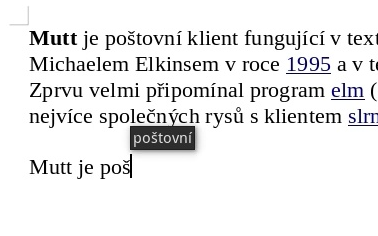
\includegraphics[width=0.5\textwidth]{LO_prediction_1}
	\caption{Implementace predikce textu v~LibreOffice Writer 4.2.8.2}
	\label{fig:LOpredict}
\end{figure}

Lze tedy říci, že nabídka slov, která daný systém vyhodnotil jako vhodná doplnění, by neměla být obtěžující, mělo by být snadné ji ignorovat a~měla by se nacházet co nejblíže místu, kam je soustředěna uživatelova pozornost. To se, jak bylo naznačeno výše, může lišit v~závislosti na cílové kategorii uživatelů.

\chapter{Smysl automatického doplňování pro uživatele}

\section{Predikce jako způsob zjednodušení zápisu}

Důvody, pro které si může uživatel vybrat užívat predikce textu, se liší podle přístroje, na němž píše, a~dalších okolností. Na mobilních zařízeních, která disponují nejednoznačnou klávesnicí (typicky starší mobilní telefony s klávesnicí ITU, tedy typickou 12tlačítkovou klávesnicí), je predikce výhodná proto, že umožňuje zadávat text jediným stisknutím kláves, které reprezentují znaky obsažené v~psaném slově. Bez predikce by byl uživatel nucen v~případě písmene, které na klávese není na první pozici, stisknout tutéž klávesu vícekrát po sobě\footnote{Více o~klávesnicích ITU v~kapitole \ref{itu-kb}.}.

Dalším případem jsou mobilní zařízení, která mají dotykový displej, kde je zase problém s~přesností, s~jakou je uživatel schopen se na klávesy trefit prstem nebo stylem. Tento případ sice spadá do kategorie automatických oprav, ale může být kombinován s~predikcí textu. \parencite{kocienda2012method} % cit. http://patft.uspto.gov/netacgi/nph-Parser?Sect1=PTO1&Sect2=HITOFF&d=PALL&p=1&u=%2Fnetahtml%2FPTO%2Fsrchnum.htm&r=1&f=G&l=50&s1=8232973.PN.&OS=PN/8232973&RS=PN/8232973 --background || tahle citace, from now on: applePatent01
	% Done

Při psaní na jednoznačné fyzické klávesnici (typicky klasická klávesnice QWERTY, jež je pro jednoduchost v~této práci považována za reprezentanta všech ostatních lokalizovaných rozložení) obvykle není predikce potřeba, ale například pro uživatele handicapovaného může být výhodné mít k~dispozici systém, který mu ušetří stisky kláves nutné k~zapsání celého slova.

\section{Predikce jako inspirace}

Vedle původního určení predikce textu, kterým je zrychlit zadávání textu a~tím komunikaci na rozhraní člověk--počítač, může pro běžného uživatele automatické doplňování textu plnit ještě několik dalších funkcí.

Takovým případem může být doplňování ve vstupním poli vyhledávače typu Google, případně jeho obdoby v~nějaké menší síti, například na elektronickém portálu knihovny. \parencite{google2015}

\textcite{ward2012autocomplete} uvádí, že studenti, na kterých testoval automatické doplňování ve vyhledávání v~rámci informačního systému knihovny, poukázali v~následném dotazníku na několik dalších funkcí, které pro ně predikce plnila.

Na otázku, jak by svým přátelům vysvětlil, k~čemu je našeptávač dobrý, odpověděl jeden student, že rozhodně jako asistence v~pravopisu. Studenti totiž často nemají z~ústních zadání v~hodinách úplně přesnou představu, jak se např. jméno autora, jehož díla jim jejich vyučující doporučil jako zdroj informací k~práci, přesně píše. Autoři studie ze záznamů hledání vyvodili, že někteří studenti si ani nemuseli být vědomi faktu, že začátek jména autora zadali špatně, protože predikce jim nabídla rovnou správnou verzi a~oni ji vybrali, aniž by přemýšleli, v~čem se nabídka liší od jejich vstupu. 

Mezi další výhody, které studenti uvedli ve zmíněné studii, patřilo například to, že automatické doplňování jim potvrdilo, že podobné téma již někdo před nimi hledal a~jejich postup je tedy pravděpodobně správný. 

S tímto souvisí i~jedna odpověď od dalšího účastníka studie, která uvádí, že našeptávač pro něj fungoval jako nástroj pro dotvoření myšlenky, jako brainstorming od počítače. 

Z výše uvedeného lze tedy vyvozovat, že automatické doplňování textu na klasickém počítači skutečně nemá význam pouze pro uživatele tělesně či jinak handicapované, kteří mohou mít problém se samotným zadáváním textu, ale může posloužit i~běžným uživatelům jako nástroj pro kontrolu toho, zda to, co píšou, je správně, k~tématu a~podobně. Základním rozdílem oproti předchozím případům využití predikce je fakt, že uživatel nemusí přesně vědět, co chce napsat, před tím, než to vidí jako doplnění.
% cit. autocomplete_as_a_research_tool.pdf
	% Done

\chapter{Jak predikce textu funguje}

\section{Slovníkový model}

Pokud prediktivní systém využívá slovníkového modelu, znamená to, že má v~paměti zařízení uložený slovník (seznam slov) společně s~jejich frekvencemi v~referenčním korpusu, tedy tzv. frekvenční slovník\footnote{Více o~frekvenčních slovnících v~kapitole \ref{frecdic}}. % cit. http://lifehacker.com/how-predictive-keyboards-work-and-how-you-can-train-yo-1643795640 -- searchfor:"The single thing that unites these" 
	% Done
Implementace frekvenčních slovníků v~aplikacích pro predikci textu se pravděpodobně značně liší a~vzhledem k~tomu, že jde většinou o~uzavřené komerční systémy, není možné konkrétní implementace zjistit. \parencite{alanhenry2014}

U systémů na mobilních telefonech s~ITU klávesnicí výběr kandidátského slova probíhá tak, že systém vytvoří kombinace všech slov, která mohou vzniknout z~písmen na stisknutých klávesách, a~vzniklá slova porovná se slovníkem. Průnik těchto dvou množin pak je uživateli nějakým způsobem prezentován. 

Systémy s~plnou klávesnicí QWERTY na mobilních zařízeních čelí, jak bylo naznačeno výše, jinému problému. Jelikož je velikost zařízení omezená a~klávesy jsou tudíž relativně malé, je vysoká pravděpodobnost, že se uživatel dopustí chyby při zadávání vstupu. \parencite{kocienda2012method} % cit. (opet) applePatent01 --background
	% Done

Řešení je podle \textcite{kocienda2012method} následující. Po získání vstupu z~klávesnice se vytvoří permutace, které jsou pak porovnávány se slovníkem. Permutace jsou v~tomto případě řetězce, jež byly vytvořeny tak, že pro každý znak $A$~v původním zadaném řetězci $O$~je vytvořen nový řetězec $P$~obsahující na pozici původního znaku $A$~znak $A$~nebo znak, který byl na klávesnici původnímu znaku $A$~sousedem. Pro slovo \exmp{pes} by tak vytvořené permutace při použití klávesnice QWERTY vypadaly na anglické QWERTY takto: % cit. applePatent01 -- searchfor:"Permutations of input characters and neighbor"
	% Done

\begin{center} 
	\exmp{pes, oes, les, prs, pds, pws, pss, pew, pee, pea, ped, pex, pez}
\end{center}

Dalším řešením je hledání slov ve slovníku, která mají od zadaného slova určitou editační vzdálenost. Editační vzdálenost je Levenshteinova vzdálenost, tedy vyjádření míry odlišnosti dvou řetězců minimálním množstvím operací {\bf vložit} znak, {\bf smazat} znak, {\bf prohodit} dva sousední znaky a~{\bf nahradit} jeden znak jiným, které je nutno provést, aby z~prvního řetězce byl vytvořen druhý \parencite{levenshtein-en1966}. \nocite{levenshtein1965}  % cit. https://en.wikipedia.org/wiki/Levenshtein_distance
	% Done
Tato metoda také využívá frekvenčního slovníku, který navíc kombinuje se statistickým modelem pravděpodobnosti výskytu a~pravděpodobnosti souvýskytu. \parencite{peternorvig} % cit. http://norvig.com/spell-correct.html
	% Done

\subsection{Frekvenční slovníky}\label{frecdic}

Frekvenční slovník je slovník, který ke každému heslu uvádí hodnoty spojené s~frekvencí daného slova ve zdrojovém korpusu. Obvykle to je hodnota absolutní frekvence daného slova, tedy počet výskytů všech tvarů daného slova v korpusu. Například {\it Frekvenční slovník češtiny} \parencite{vcermak2004frekvenvcni} %  cit. Čerák et al. 
vedle ní uvádí také průměrnou redukovanou frekvenci, což je hodnota, jež vychází z~absolutní frekvence, avšak zohledňuje rozložení daného slova v~korpusu. Pokud tedy mají dvě slova stejnou frekvenci, avšak první z~nich se vyskytuje pouze v~malém množství odborných textů, zatímco výskyty druhého jsou rovnoměrně rozloženy přes celý korpus, druhé slovo dostane vyšší číselnou hodnotu ARF (average reduced frequency) než slovo první. Podle hodnoty ARF tak lze vyvodit, že druhé slovo je obecně známější a~užívanější širším publikem \parencite{vcermak2004frekvenvcni}. %  cit. Frek slovník, Čermák, předmluva % Done
% cit. https://debtest.fi.muni.cz:8020/czechency?action=getdoc&amp;tr=preview2&amp;id=FREKVEN%C4%8CN%C3%8D%20SLOVN%C3%8DK  % Not Done
V~kontextu s~predikcí slov to může například znamenat, že je pravděpodobnější, že uživatel chce napsat spíše druhé slovo nežli první, které je pravděpodobně značně odborné.


Tvorba frekvenčních slovníků byla v~dobách před rozvojem počítačů schopných zpracovat velká množství textů poněkud komplikovaná. Databáze textů bylo obtížné jak vytvářet, tak aktualizovat a~jejich výroba byla náročná a~pomalá. Nástup počítačů však většinu těchto problémů odstranil, takže je možné velmi snadno z~korpusu vyrobit frekvenční slovník, který bude tak aktuální, jako je samotný korpus. Na rozdíl od ručního zpracování dat navíc počítačové zpracování dovoluje pracovat s~mnohem většími korpusy, takže výsledný frekvenční slovník může být i~přesnější. Pro srovnání, jeden z~prvních frekvenčních slovníků pro angličtinu, {\it The Teachers Word Book of 30~000~words}\footnote{učitelský slovník 30~000~slov} \parencite{lorge1944teacher}, měl 30 tisíc lemmat (z 13 tisíc slovních rodin%  cit. Goulden, Nation and Read, 1990  % Done
% Thorndike, Edward L. 1874-1949. The Teacher's Word Book of 30,000 Words. New York: Teachers College, Columbia University, 1944. -- http://catalog.hathitrust.org/Record/000987642/Home  % Done
) a~byl vyroben z~ručně psaného korpusu, který obsahoval 18 milionů slov \parencite{nation1997vocabulary}. %  cit. http://www.lextutor.ca/research/nation_waring_97.html  % Done
Naproti tomu {\it A~frequency dictionary of contemporary American English}\footnote{frekvenční slovník současné americké angličtiny} \parencite{davies2013frequency} byl vytvořen z~korpusu současné americké angličtiny, {\it The Corpus of Contemporary American English}\footnote{korpus současné americké angličtiny, \url{http://corpus.byu.edu/coca/}}, který obsahuje přes 400~milionů slov. Samotný slovník obsahuje pouze 5~000~slov, protože je určen především uživatelům, kteří nejsou rodilí mluvčí a~anglicky se učí, takže potřebují výrazně menší množství slov.
% A~Frequency Dictionary Of American English, 2010 % Done

\textcite{alderson2007judging} tvrdí, že ani velké korpusy nemusí být dostačující pro adekvátní zhodnocení frekvenčního rozložení slov v~jazyce tak, jak jej vnímají mluvčí daného jazyka. Vychází z~výsledků výzkumů zaměřujících se na porovnání hodnocení frekventovanosti určitých slov v~jazyce jeho zkušenými uživateli s~daty získanými z~korpusu. Tyto hodnoty se totiž značně rozchází a~je tedy otázkou, zda z~toho vyplývá, že ani zkušení mluvčí nedokážou správně posoudit pravděpodobnost výskytu daného slova, či že data získaná z~korpusů nereprezentují zkušenosti mluvčích s~jazykem dostatečně přesně.
% http://applij.oxfordjournals.org.ezproxy.muni.cz/content/28/3/383.full
	% Done

% \begin{spacing}{1.07}
\section{Statistický model}

Statistické modelování je založeno na výběru predikce na základě pravděpodobnosti, s~jakou se řetězec může vyskytnout v~jazyce a~případně v~daném kontextu. \parencite[5233]{ghayoomi2009overview}

Řetězcem mohou být jednotlivá písmena či celá slova. V~případě jednotlivých písmen má systém uložen databázi n-gramů s~jejich frekvenčním rozložením, z~nichž pak vybírá ty, které mají shodný prefix s~již zadaným textem. Práce s~celými slovy probíhá podobně, ale jako databázi má systém uložen frekvenční slovník. 

Hranice mezi statistickým a~slovníkovým modelem není v~tomto případě zcela pevná, protože slovníkový model také využívá frekvenčního slovníku a~rozdíl se tak smazává. Například \textcite[5234]{ghayoomi2009overview} slovníkový model neuvádí samostatně, ale řadí jej pod statistické modelování. Z~hlediska této práce se však jevilo vhodnějším modely rozdělit, aby tak lépe vynikl rozdíl mezi jednotlivými metodami predikce textu, které jsou uvedeny v~kapitole \ref{input-methods}.

\section{Model se znalostní bází}

Často se stává, že návrhy učiněné aplikacemi se slovníkovým či statistickým modelem jsou v~daném kontextu nevhodné a~mnohdy i~negramatické. Tento problém se snaží řešit systémy, které kombinují další metody zúžení výběru návrhů. 

Gramatické správnosti lze docílit využitím syntaktické analýzy zadaného řetězce (věty) a~využitím n-gramů slovních druhů vytvořených z~korpusu (jinými slovy databáze pravděpodobností, že slovní druh $X$~je následován slovním druhem $Y$). Tento model může dále využívat gramatiky pro generování korektních vět. \parencite[5234--5235]{ghayoomi2009overview}

Aby bylo docíleno kontextové správnosti návrhů, je nutno zapojit do predikce i~sémantickou analýzu. Pro takovou analýzu je možno využít například rozsáhlé sémantické sítě Wordnet\footnote{\url{https://wordnet.princeton.edu/}}. \parencite[5235]{ghayoomi2009overview}

Jakkoliv gramaticky správná a~sémanticky vhodná, predikce stále nemusí být pro uživatele použitelná, protože je v~rozporu s~diskursem. Pro eliminaci takových situací může systém využívat korpus obsahující pragmatická data a~vyřadit z~výběru slova, která jsou pravděpodobně nevhodná. \parencite[5235]{ghayoomi2009overview}

\section{Heuristický model}

Heuristické modely jsou takové, které se buď v~dlouhodobém, nebo krátkodobém měřítku adaptují konkrétnímu uživateli. Činit tak mohou analýzou textu, který v~minulosti uživatel zadal, a~podle toho uzpůsobovat další predikce. Uzpůsobením se rozumí například upřednostnění slov, která již uživatel zadal před těmi, jež ještě nikoliv. \parencite[5235]{ghayoomi2009overview}

Aplikace popisovaná v~této práci jistým způsobem využívá heuristického modelování, protože preferuje určitá již uživatelem zadaná slova před predikcemi vrácenými serverovou částí aplikace.
% \end{spacing}

\chapter{Měření účinnosti zadávání textu}

Vstupní metody mívají zpravidla dva cíle, jichž se snaží jejich vývojáři dosáhnout. Jedním z~nich je omezení počtu nutných úhozů při zadávání textu, druhým pak je rychlost samotného zadávání. Omezování počtu nutných úhozů je aktuální u~nejednoznačných klávesnic, které zpomalují zadávání textu především nutností stisknout jednu klávesu vícekrát pro zadání některých znaků. Tento problém u~jednoznačných klávesnic QWERTY není tak podstatný, takže záleží spíše na rychlosti zadávání.

Měřit rychlost zadávání textu pak lze několika odlišnými způsoby. Uživatelé, na kterých se testuje, mohou buď psát text předem nepřipravený, tedy ho mohou komponovat sami, nebo mohou kopírovat již hotový text. Kopírování se obecně považuje za lepší, protože eliminuje zpoždění nutné k~samotnému vymyšlení psaného textu. \parencite[2]{tarvainen2010beginner} % cit. gradu04481.pdf ch 1.1 text entry evaluations & Arif ch 2~- text entry perf. metrics
	% Done

\section{Měření počtu úhozů na znak}

Metoda měření počtu úhozů na znak, neboli KSPC\footnote{Přestože název obsahuje stisky kláves, veličina se používá i~pro měření účinnosti zadávání textu např. pomocí stylu na dotykovém zařízení.} (keystrokes per character), je nejužitečnější metrikou pro vyhodnocování těch metod zadávání textu, které se snaží o~snížení množství úhozů na znak, jako  je například prediktivní systém T9\footnote{Více o~predikci T9 v~kapitole \ref{t9}.}. KSPC tedy udává průměrný počet úhozů nutný k~zadání jednoho znaku.

\subsection{Primitivní výpočet}

Naivní přístup k~výpočtu KSPC je takový, že se spočítá počet písmen ve slově (i s~mezerou za slovem) a~počet úhozů, kterými se na dané klávesnici slovo zadá. Nutno počítat i~se stisky speciální klávesy \exmp{NEXT}, kterou je nutno použít v~případě, že se dvě po sobě jdoucí písmena nachází na stejné klávese \parencite[10]{silfverberg2000predicting}. % cit Silfverberg, M., MacKenzie, I. S., and Korhonen, P. Predicting text entry speed on mobile phones, Proc. CHI 2000. New York: ACM (2000) 9-16.
	% Done
Pro metodu multitap na standardní ITU klávesnici by to pro slovo \exmp{kniha} byla následující sekvence kláves:

\[
	\exmp{kniha\_: 5566444N442S},
\]
kde \exmp{N} je \exmp{NEXT} a~\exmp{S} je znak mezery. KSPC vypočteme jako poměr úhozů na znak:

\[
	\frac{12}{6} = 2,000.
\]
Je ovšem evidentní, že pokud se nyní stejným způsobem provede výpočet pro slovo \exmp{data}, bude sekvence úhozů mnohem jednodušší:

\[
	\exmp{data\_: 3282S}
\]
a KSPC tedy vyjde:

\[
	\frac{5}{5} = 1,000.
\]

Z toho vyplývá, že je nutno provést výpočet tak, aby výsledná hodnota byla průměrná pro daný jazyk. Takový výpočet má dvě prerekvizity. První z~nich je jednoznačný popis postupu, kterým lze dojít k~zadání jednotlivých znaků, druhou pak jazykový model. Ten je nutný proto, aby výsledné KSPC bylo nezávislé na konkrétním textu v~daném jazyce (tedy aby pro daný jazyk bylo průměrné). \parencite[196]{mackenzie2002kspc}

\subsection{Jazykový model}

Jazykovým modelem je v~případě měření KSPC korpus a~jeho omezené formy. Tyto formy se liší podle toho, jaká metoda zadávání je testována. Pokud například jde o~metodu, která vybírá znaky nezávisle na kontextu, stačí mít informace o~frekvenčním rozložení jednotlivých písmen v~korpusu. Pokud by byl výběr znaku závislý na kontextu jednoho písmene, byl by jazykový model frekvenční slovník bigramů. Pro vyhodnocení metod, které využívají k~odhadu dalšího písmene kontext celých slov, se použije korpus zredukovaný na unikátní slova a~jejich frekvence.  \parencite[197]{mackenzie2002kspc} % cit. MacKenzie ch 4.3 % Done

\subsection{Obecný výpočet}

Při výpočtu průměrného KSPC pro daný jazyk a~metodu se pak postupuje podle následujícího vzorce:

\[
	KSPC = \frac{\sum{ (K_c \times F_c) }}{\sum{ (C_c \times F_c) }},
\]
kde $K_c$ je počet úhozů nutných pro zadání znaku, $C_c$ je velikost znaku a~$F_c$ je frekvence daného znaku v~korpusu. Pokud se tedy tento vzorec aplikuje na situaci, kdy metoda zadávání textu vybírá písmeno bez ohledu na kontext, platí, že $C_c$ = 1, pokud se vybírá v~závislosti na jednom předešlém znaku, je $C_c$ = 2. Pokud metoda zohledňuje celá slova, počítá se s~průměrnou délkou slov v~daném jazyce. Ta se počítá jako vážený průměr počtu znaků ve slovech daného jazyka, který pro BNC\footnote{Britský národní korpus, \url{http://www.natcorp.ox.ac.uk/}} vychází na 4,59 znaku; pro srovnání, \textcite[2]{arif2009analysis} počítají při svých výpočtech s~5 úhozy na slovo, což se považuje za obecný standard. \parencite[3]{tarvainen2010beginner} % cit. gradu04481.pdf ch. 1.1.1 WPM & Arif ch 2~- text entry perf. metrics - WPM 
	% Done (both)

\subsection{Obecné dělení metod zadávání dle počtu úhozů na znak}

Metody zadávání textu lze podle KSPC rozdělit do tří kategorií: ty, pro které je KSPC větší než 1~(např. původní metoda multitap), ty, pro které je rovno 1~(např. klávesnice QWERTY) a~nakonec ty, jejichž KSPC dosahuje hodnot nižších než 1~(např. klávesnice QWERTY kombinovaná s~predikcí). % cit. MacKenzie KSPC ch. 2~a MacKenzie KSPC ch. 6

Jako základ pro porovnání jednotlivých metod podle KSPC je vhodná standardní klávesnice QWERTY \parencite{arif2009analysis}. % Arif - introduction
Uvažují-li se pouze malá písmena anglické abecedy, platí pro ni, že KSPC = 1, tedy na jeden znak připadá jeden úhoz, protože pro každý znak má dedikovanou právě jednu klávesu.

\section{Měření počtu slov za minutu}

Počet slov za minutu (WPM, Words per minute) je běžně užívaná metrika pro vyhodnocení rychlosti psaní \parencite{tarvainen2010beginner}. % cit. gradu04481 ch. 1.1.1
Tato metoda nezohledňuje počet úhozů, který byl během měření proveden, pouze výslednou délku přepsaného řetězce. Vzorec pro výpočet WPM \parencite[48]{wobbrockjacobo.2007}:

\[
	WPM = \frac{T - 1}{S} \times 60 \times \frac{1}{5},
\]
kde $T$ je délka přepsaného řetězce, $S$ počet sekund od prvního úhozu do posledního úhozu. Konstanta $60$ reprezentuje počet sekund za minutu a~$1/5$ počet znaků na slovo. Aby byla metoda univerzální, počítá se slovo jako pět znaků nezávisle na tom, kolik znaků slova ve výsledném řetězci skutečně mají. Tato standardizace se vyskytuje už od roku 1905 \parencite{yamada1980historical}. Odečtení konstanty $1$ z~počtu znaků ve výsledném řetězci je důležité proto, že většina systémů začíná počítat čas ve chvíli zadání prvního znaku. \parencite[49]{wobbrockjacobo.2007}

\section{Vyhodnocování chyb}

Při vyhodnocování rychlosti psaní je důležité zohlednit také chyby ve výsledném textu, jelikož jinak by bylo možné dosáhnout velice dobrých výsledků pouhým rychlým náhodným mačkáním kláves.

Metoda KSPC může být použita k~vyčíslení chybovosti tak, že porovná počet znaků zadaných a~počet znaků ve výsledném řetězci. Jednou z~nevýhod je fakt, že žádným způsobem nerozlišuje chybné znaky od správných, takže vyčísluje pouze množství oprav. % gradu04481.pdf ch 1.1.4 about error rates

Dalším způsobem, jak změřit chybovost, s~jakou uživatel text zadal, je vyhodnocení Levenshteinovy vzdálenosti originálního a~přepsaného řetězce. \parencite{soukoreff2001measuring} % cit gradu04481.pdf ch 1.1.4

\chapter{Rozšířené metody zadávání textu}\label{input-methods}

\section{Klávesnice ITU}\label{itu-kb}

Klávesnice ITU je textová klávesnice na tónovém telefonu, která má na jednu klávesu přiřazeno více písmen. V~průběhu vývoje se vyskytovalo několik různých způsobů, jak byla písmena na klávesnici rozřazena, podle mezinárodního standardu ITU E.161/ISO 9995-8 je rozložení následující: % cit norma ITU E.161/ISO 9995-8 
% \cite{mfmtlqoxL48pMk3T}
% TODO: nejsem schopen to v~tom dokumentu najit - http://www.itu.int/rec/T-REC-E.161/en

\begin{figure}[h]
	\centering
	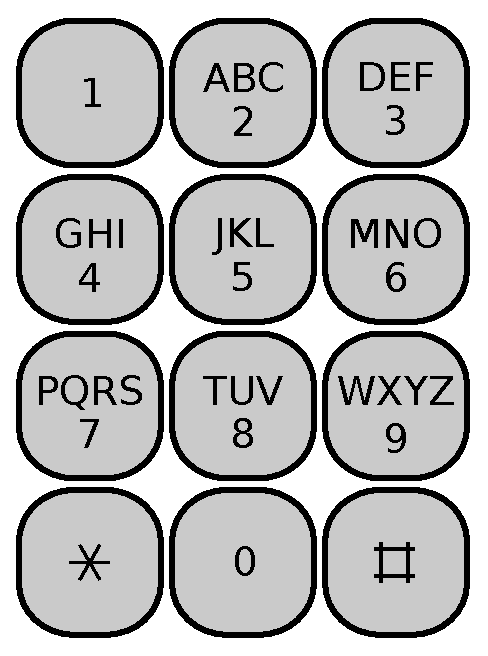
\includegraphics[width=0.4\textwidth]{telephone-keypad.eps}
	\caption{Klávesnice ITU (ISO 9995-8)\protect\footnotemark}
	\label{fig:phoneKeyboard}
\end{figure}

\footnotetext{Převzato z~Wikimedia Commons}

\subsection{Multitap}

Na těchto klávesnicích musí uživatel stisknout klávesu s~požadovaným písmenem tolikrát, jaké je pořadí daného písmena na klávese. Například na klávese \exmp{3} jsou písmena \exmp{D}, \exmp{E}, \exmp{F}, tudíž chce-li uživatel zadat písmeno \exmp{F}, musí klávesu \exmp{3} stisknout třikrát. Např. pro napsání slova \exmp{nejlepsi\_} tak je nutno stisknout 21 kláves:

\[
	\exmp{nejlepsi: 66335N555337N7777444S}.
\]

Tento systém zadávání se nazývá multitap podle toho, že na jeden znak připadá několik úhozů. Při psaní tímto systémem může KSPC dosahovat hodnot přes 2, protože většina kláves musí být stisknuta vícekrát než jednou. \parencite[202]{mackenzie2002kspc}

Aby bylo možné zbavit se tohoto problému u~klávesnic, které mají méně kláves, než je písmen v~abecedě, je nutné nějakým způsobem disambiguovat vstup vzniklý tak, že uživatel stiskl klávesy, na nichž se vyskytovala potřebná písmena, vždy jen jednou. Termín predikce textu je v~tomto případě poněkud nepřesný, ale je použitelný, protože systém na základě nejednoznačného vstupu předvídá, odhaduje, co uživatel chtěl napsat. Toto odhadování může být prováděno dvěma způsoby -- na základě slovníku a~na základě prefixů.

\subsection{Slovníková disambiguace}

Slovníková disambiguace umožňuje uživateli zadávat text jediným stiskem každé klávesy s~požadovaným písmenem. Systém potom vyhledává ve slovníku záznamy korespondující se sekvencí stisknutých kláves, tzn.~slova, která obsahují písmena ze stisknutých kláves. Pokud sekvenci stisknutých kláves odpovídá více slov, je uživateli prezentován seznam těchto slov seřazený obvykle podle frekvence výskytu. % http://patft.uspto.gov/netacgi/nph-Parser?Sect1=PTO1&Sect2=HITOFF&d=PALL&p=1&u=%2Fnetahtml%2FPTO%2Fsrchnum.htm&r=1&f=G&l=50&s1=6011554.PN.&OS=PN/6011554&RS=PN/6011554

Tento způsob disambiguace samozřejmě není dokonalý, protože mnoho různých slov sdílí stejné kombinace kláves. V takovém případě pak uživatel musí pomocí speciálních kláves požadované slovo vybrat \parencite{MacKenzie2001}. Například kombinace kláves \exmp{7725} má v~češtině možné min. tři interpretace: \exmp{prak, pral, psal}.

Slova, která se zapisují stiskem stejných kláves, se nazývají textonyma \parencite{ericzorn2007} a v~angličtině jsou jimi např. slova \exmp{book} a~\exmp{cool}. Zatímco obvykle tento jev pouze snižuje efektivitu zápisu textu, v~roce 2010 záměna dvou textonym v~textové zprávě vedla ve Spojených státech k~vraždě. \parencite{t9kill}

\subsubsection{První disambiguační systém} 

První disambiguační systém byl určen pro lidi s~částečně nebo zcela poškozeným slyšením. Tento systém, navržený v~roce 1985, si kladl za cíl umožnit neslyšícím telefonní komunikaci, a~to za přijatelnou pořizovací cenu (na rozdíl od předchozích existujících řešení) a~s tím, že speciální přístroj bude potřebovat pouze neslyšící strana. \parencite{feinson1988interpretive}

Zpráva se neslyšící straně předává tak, že protistrana na svém přístroji stiskne pro každé písmeno ve zprávě klávesu, na níž se písmeno vyskytuje (a to pouze jednou), tyto stisky se převedou na tón o~odpovídající frekvenci (podobně jako u~tónové volby) a tón se přenese po telefonní lince neslyšící straně. Tam je sekvence tónů převedena pomocí přístroje vybaveného mikroprocesorem na sekvenci skupin znaků, které odpovídají daným klávesám, a~provede se prohledání slovníku lokálně uloženého v~přístroji. Nalezená shoda je pak uživateli zobrazena na obrazovce telefonního přístroje.

\subsubsection{T9}\label{t9}

T9 -- akronym pro {\it Text on 9~keys} -- je systém, který se společně s~větším rozvojem mobilních telefonů s~klasickými 12klávesovými klávesnicemi se stal všeobecně známým pojmem pro predikci textu. Byl vyvinut společností Tegic Communications, jež později přešla pod firmu Nuance Communications \parencite{nuancecommunications2007}, a patentovaný ve Spojených státech \parencite{grover1998reduced}. 

Systém T9 umožňuje uživateli rozšiřovat vestavěný slovník tak, že uživatel nové slovo zadá klasickým způsobem multitap a~nové slovo se pak uloží do uživatelské databáze \parencite{t9about}. % http://www.nuance.com/for-business/by-product/t9/index.htm
Problém nastává ve chvíli, kdy uživatel zjistí, že slovo není ve slovníku, až poté, co zadá příslušnou sekvenci kláves, která by k~onomu slovu měla vést. V~tu chvíli totiž musí smazat zadaný řetězec, který je buď nesmyslný, nebo to není požadované slovo, a~zadat slovo znova pomocí multitapu.

Celkově je však T9 velmi jednoduchá na pochopení a~použití a~pro její nezávislost na kontextu u~ní lze očekávat vždy stejný výstup po stisknutí určité sekvence kláves, takže se zkušený uživatel nemusí při psaní dívat na klávesnici. \parencite{davidmackay}

\subsubsection{iTap}

Firma Motorola vyvinula iTap jako systém konkurenční k~systému T9. Přestože oba systémy využívají slovníkového modelu, iTap je na rozdíl od T9 kontextově závislý a~jeho slovník obsahuje kromě jednotlivých slov i~běžně užívané fráze. 

\textcite{davidmackay} dále uvádí, že ve srovnání se systémem T9 je systém iTap pro uživatele méně výhodný v~tom smyslu, že jsou nuceni činit rozhodnutí ohledně toho, zda v~určitém momentu zvolit nabízenou predikci, či pokračovat v~manuálním psaní. Pro nezkušené uživatele navíc může u~systému iTap být demotivující, když jim predikce nabídne slova, která nemínili napsat. Systém iTap je také celkově mírně náročnější na ovládání.
% http://www.inference.phy.cam.ac.uk/itprnn/itap/ % Done

\subsection{Prefixová disambiguace}

\subsubsection{LetterWise}

LetterWise je systém prediktivního psaní vyvinutý a~patentovaný firmou Eatoni Ergonomics. Tento systém nepracuje se slovníkem, ale s~databází pravděpodobností prefixů pro každý používaný jazyk. Které písmeno ze stisknuté klávesy zvolit tedy systém vybírá porovnáním pravděpodobností, s~jakými mohou písmena z~dané klávesy následovat po předcházejících písmenech. V~angličtině je například nepoměrně pravděpodobnější, že po sekvenci písmen \exmp{T} a \exmp{H} bude následovat při stisku klávesy \exmp{3} písmeno \exmp{E}, nikoliv \exmp{D} či \exmp{F}. Prediktivní systém LetterWise má tedy v~paměti zařízení uloženy pouze tyto pravděpodobnosti, nikoliv celá slova. \parencite{MacKenzie2001} Díky tomu je paměťová náročnost systému LetterWise velmi nízká a~navíc jeho účinnost nedegraduje se snižující se velikostí jazykového modelu tolik, jako např. u~systému T9. Jazykový model pro šest jazyků (angličtina, dánština, italština, španělština, francouzština, němčina) zabíral na implementaci pro procesor Intel 80C51 pod 5~kB. \parencite{eatoniletterwisereq} % https://web.archive.org/web/20120212172428/http://www.eatoni.com/wiki/index.php/FAQ:For_Manufacturers

Další, pro uživatele výrazně citelnější výhodou oproti slovníkovým systémům, je možnost relativně jednoduše zapisovat i~neslovníková slova. Pokud se totiž uživatel pokouší zadat slovo, které by sice ve slovníku neexistovalo, ale má skladbu hlásek odpovídající jazyku, jehož databáze prefixů je aktivní, je pravděpodobné, že systém vybere správné písmeno. Není tedy nutné se při zápisu neslovníkových slov uchylovat k~multitapu, pouze k~jeho zmírněné verzi: čím odlišnější je slovo od aktivního jazykového modelu, tím častěji bude odhad písmene chybný a~uživatel bude muset stisknout klávesu vícekrát, aby zvolil správné písmeno. Tento systém tedy uživatele nenutí v~případě zjištění, že jím požadované slovo není ve slovníku, celé slovo smazat a~zadat jej klasickým způsobem. \parencites[5234]{ghayoomi2009overview}[112]{MacKenzie2001}

\subsubsection{WordWise}

Méně známý systém od firmy Eatoni Ergonomics, WordWise, je podobný systému LetterWise. WordWise je však na rozdíl od systému LetterWise založený na doplňování slov ze slovníku, v~čemž je podobnější systému T9. Od toho se ale liší tím, že se vrací k~systému LetterWise, pokud se uživatel pokusí zadat slovo, které nemá WordWise ve slovníku. U~LetterWise, jak je uvedeno výše, záleží počet nutných stisků kláves na podobnosti slova s~právě používaným jazykovým modelem. \parencite{eatoniwordwise}

Modifikací tohoto systému je také systém WordWise Shift, který využívá jednu klávesu na telefonu jako klávesu Shift, a~na každé klávese se skupinou písmen je vybráno jedno písmeno, jež lze napsat pouze se stiskem klávesy Shift a~dané klávesy. Toto má podle výrobce za cíl minimalizovat problémy s~predikcí slov, která sdílejí stejnou kombinaci kláves. Společnost Eatoni na svých stránkách uvádí, že uživatel při používání tohoto systému nemusí vůbec sledovat display svého zařízení, a~přesto  může jím napsaný text být zcela správně, protože chyba v~predikcích slov nastává jednou za 440 slov. \parencite{eatoniwordwise}

Paměťová náročnost jazykového modelu pro angličtinu je v~aplikaci WordWise zhruba 75 kB. \parencite{eatoniwordwise} % https://web.archive.org/web/20120212172428/http://www.eatoni.com/wiki/index.php/FAQ:For_Manufacturers % Done

\section{Klávesnice QWERTY na chytrých telefonech}

S rozvojem chytrých telefonů s~velkými dotykovými obrazovkami se do širšího používání dostaly plné klávesnice QWERTY. Tyto klávesnice, které se zobrazují na displeji zařízení, a~nemají tudíž po hmatu rozlišitelné klávesy, se také nazývají soft keyboards nebo softwarové klávesnice.

Pokud by se účinnost takové klávesnice jako metody vstupu textu porovnávala pouze podle hodnoty KSPC, byly by plné klávesnice QWERTY na chytrých telefonech stejně účinné jako standardní klávesnice k~počítačům. Realita je ovšem jiná, protože velikost klávesnic na chytrých telefonech je v~řádu centimetrů namísto desítek centimetrů, a~také proto, že na rozdíl od fyzické klávesnice nejsou jednotlivé klávesy na dotykovém displeji rozpoznatelné po hmatu. Zadávání textu na takové klávesnici proto vyžaduje ze strany uživatele větší zkušenosti a~pozornost. Text navíc nemůže zadávat všemi deseti prsty, ale při nejlepším dvěma prsty, což rychlost psaní také rapidně snižuje. Nemožnost poznat hranice kláves po hmatu navíc vede k~zásadnímu nárůstu chybovosti (překlepů), které je uživatel nucen opravovat. Ačkoliv je pravděpodobně nereálné snažit se bez empirického výzkumu zahrnout tyto faktory do teoretického výpočtu KSPC pro tyto klávesnice, lze logickým úsudkem dospět k~tomu, že i~pro tuto metodu vstupu je žádoucí zvýšit rychlost a~účinnost zadávání nějakým typem predikce textu.

\subsection{Barevné zvýrazňování kláves}

Jedním z~navrhovaných způsobů, jak pomoci uživatelům snížit množství překlepů při psaní na softwarových klávesnicích QWERTY, bylo barevně odlišovat nejpravděpodobnější následující klávesy \parencite{danielgoncalves}. % http://web.ist.utl.pt/~daniel.j.goncalves/research/paelife\_textentry/paelife\_textentry.html
Tento způsob byl navržen především pro starší uživatele, kteří jednak nemusejí být seznámeni s~rozložením klávesnice QWERTY, a~jednak nemají takovou přesnost motoriky a~rychlost reakcí, jako uživatelé mladí. 

\begin{figure}[ht]
	\centering
	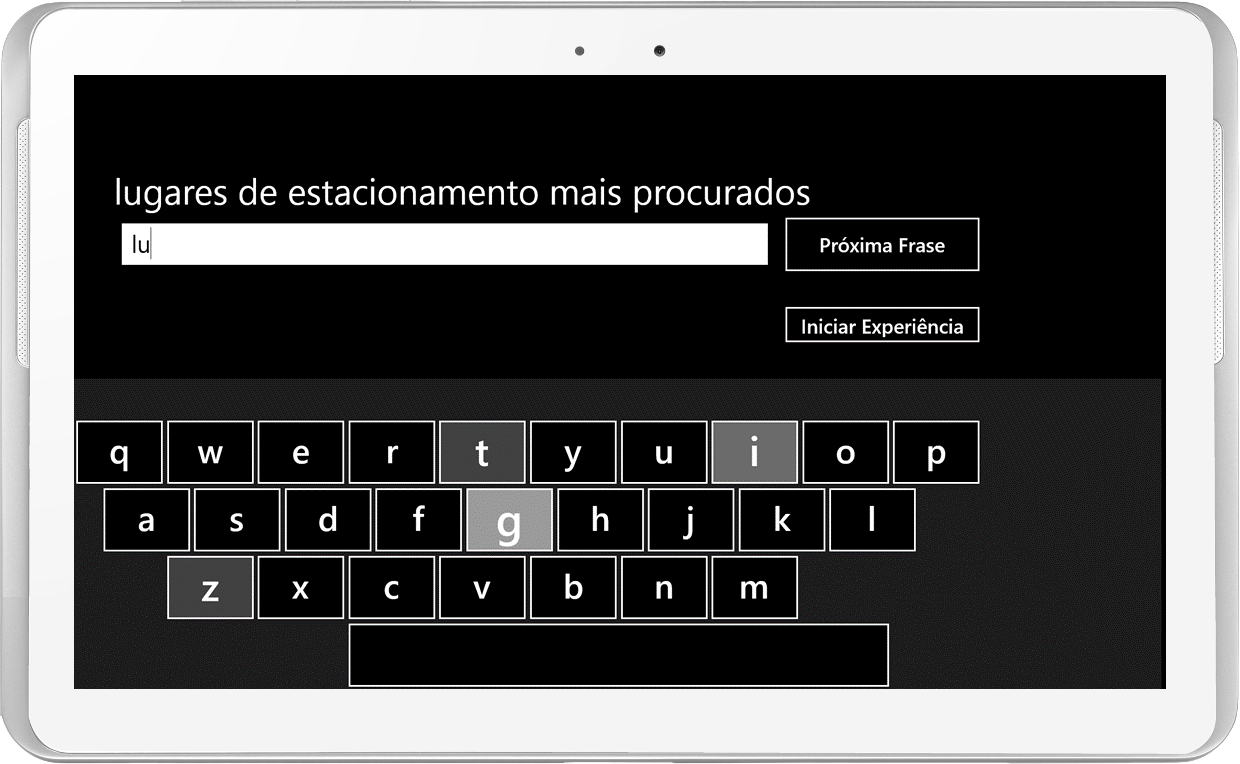
\includegraphics[width=0.4\textwidth]{qwerty_color}
	\caption{QWERTY -- barevné zvýrazňování}
	\label{fig:qwerty-color}
\end{figure}

Klávesy byly odlišeny různými odstíny šedé barvy, a~to lineárně podle toho, jak pravděpodobné bylo dané písmeno v~souvislosti s~předchozím zadaným znakem. Vedle barevného odlišení pozadí klávesy byl ještě zvětšen popisek klávesy (obrázek \ref{fig:qwerty-color}). 

Výsledky studie, která byla provedena na 15 ženách a~5 mužích, ovšem předpoklad, že zvýrazňování kláves starším uživatelům pomůže, popřely. Ukázalo se, že snaží-li se klávesnice vizuálně nějakým způsobem odlišit některé prvky a~přitáhnout k~nim pozornost uživatele, působí to na něj spíše rušivě a~výrazně to snižuje rychlost zadávání textu. Jeden uživatel dokonce napsal místo slova, které zamýšlel, slovo, které mu nabízela predikce. Funkčnost systému zvýrazňování navíc byla omezena tím, že starší uživatelé dělali v~textu hodně chyb a~systém pak nebyl schopen správně rozpoznat daná slova.
% TODO: cisla z~clanku nebudou, protoze jim actually nerozumim xD http://goo.gl/1G8wGB (mam na mysli ty typu "(F(2,30)=3.84, p< 0.033)")

\subsection{Predikce celých slov}

Druhým navrhovaným způsobem ve výše zmíněné studii byla metoda, kterou používá v~současné době většina klávesnic na chytrých telefonech.

Jde o~systém, kde po zadání znaku či znaků je ze slovníku známých slov vybráno několik slov, která jsou v~souvislosti s~již zadanými znaky nejpravděpodobnějšími řetězci, jež uživatel chce zadat (obrázek \ref{fig:qwerty-predict}). Tento seznam je obvykle nabízen ve formě horizontálního seznamu nad klávesnicí a~uživatel může ušetřit několik stisků kláves tak, že vybere požadované slovo ještě před tím, než jej celé dopíše (za předpokladu, že jej systém našel ve svém slovníku a~správně navrhl). 

\begin{figure}[ht]
	\centering
	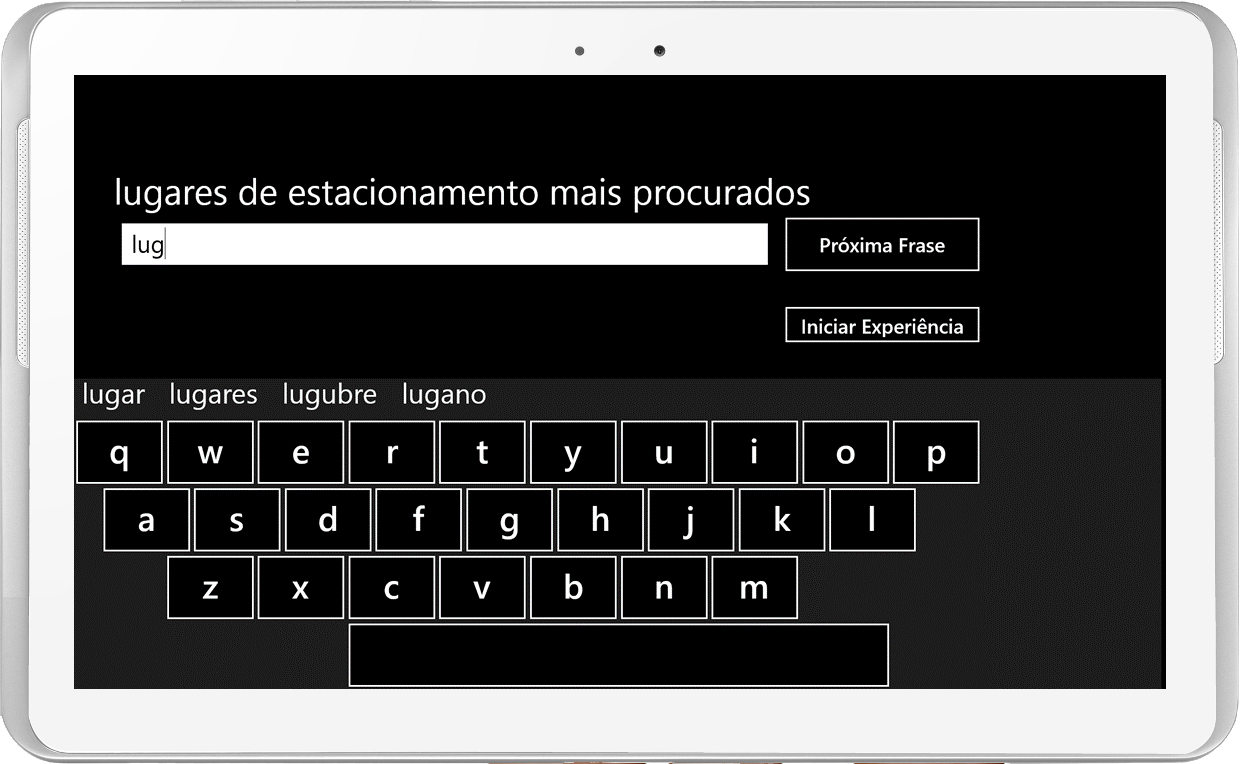
\includegraphics[width=0.4\textwidth]{qwerty_predict}
	\caption{QWERTY -- seznam predikcí}
	\label{fig:qwerty-predict}
\end{figure}

Oproti zvýrazňování jednotlivých nejpravděpodobnějších kláves má tento systém minimálně dvě výhody. Jednak nevyžaduje, aby si uživatel nestínil prsty, kterými píše, výhled na klávesnici, a~jednak uživateli zobrazuje celá slova, ne pouze další znak z~nich.

Nevýhodou této metody na druhou stranu je fakt, že je na uživatele kladena vyšší kognitivní zátěž v~tom smyslu, že je nucen procházet zrakem seznam navrhovaných slov a~přemýšlet, zda je mezi nimi i~to, které zamýšlel napsat. Z~tohoto důvodu je nutné délku seznamu návrhů omezit na optimum. Například \textcite{neverilovaulipova2014} ve své implementaci používají šest návrhů a~implementace popisovaná v~praktické části této práce používá pět návrhů.

\subsection{Swype}

Další systém zadávání textu, který je poněkud odlišný od všech dosud zmíněných, používají mj. aplikace Swype\footnote{\url{http://www.swype.com/}}, Fleksy\footnote{\url{https://fleksy.com/}}, oficiální klávesnice od Google, etc. Jde o~systém původně vyvinutý firmou Swype Inc. určený výhradně pro dotyková zařízení. Uživatel v~něm nezadává text ťukáním na jednotlivé klávesy, ale přejíždí prstem či stylem po klávesnici od prvního písmena zadávaného slova k~poslednímu tak, aby na cestě přejel pokud možno přes všechna písmena obsažená ve slově. \parencite{swypeabout} % http://www.swype.com/product-features/android/features.html
% http://patft.uspto.gov/netacgi/nph-Parser?Sect1=PTO1&Sect2=HITOFF&d=PALL&p=1&u=%2Fnetahtml%2FPTO%2Fsrchnum.htm&r=1&f=G&l=50&s1=7,098,896.PN.&OS=PN/7,098,896&RS=PN/7,098,896

Swype se skládá ze tří základních částí -- analyzátoru trasy dotyku, systému na vyhledávání slov v~databázi výrazů a~uživatelského prostředí \parencite{kushler2006system}. V~raných verzích databáze obsahovala 65 000 výrazů. \parencite{rafeneedleman2008} % % http://www.cnet.com/news/move-over-t9-here-comes-swype/ % Done

Nutno podotknout, že firma Nuance, jež systém Swype v~současnosti vyvíjí, nezahrnuje do své klávesnice pouze tento systém zadávání, ale i~klasickou metodu zadávání s~nabídkou predikcí v~horizontálním seznamu. Navzdory faktu, že hlavním důvodem popularity klávesnicové aplikace Swype je systém zadávání Swype, i~klasická klávesnice v~této aplikaci kombinuje různé technologie na zlepšení uživatelského komfortu. Mezi ně patří například schopnost rozšiřovat virtuální (nikoliv vizuální) velikost klávesy podle toho, jaké klávesy předcházely. Pokud uživatel tedy např. často klepne na klávesu \exmp{N}, smaže zadaný znak \exmp{N} a místo něj napíše \exmp{B}, pak se to klávesnice naučí a~příště, pokud je klepnutí ne zcela jednoznačné, vybere pravděpodobnější klávesu, v~tomto příkladu tedy \exmp{B}. \parencite{swypeabout} % http://www.swype.com/product-features/android/features.html 

% http://www.nuance.com/ucmprod/groups/corporatecomms/@web-enus/documents/webasset/nc\_024737.pdf

Swype také používá Andvance Language Model (AML), „pokročilý jazykový model“, který pracuje s~bigramy a~trigramy vytvořenými mimo jiné na základě textů, které už uživatel zadal. To aplikaci umožňuje účinněji disambiguovat slova, která vychází jako možná řešení uživatelova vstupu, či předvídat další slovo, které by mohlo přijít po již napsaném. Oficiální dokumentace uvádí, že díky AML aplikace dokáže na základě kontextu správně rozlišit slova, která mají stejnou trasu tahu, tedy v angličtině např. \exmp{put}, \exmp{pit} a \exmp{pot}. \parencite{swypehowto}
% http://www.nuance.com/ucmprod/groups/corporatecomms/@web-enus/documents/webasset/nc\_024737.pdf

\subsection{Predikce na fyzických klávesnicích QWERTY}

Jak bylo naznačeno v~kapitolách výše, většina implementací predikce textu, automatického doplňování textu a~automatických oprav založených na predikci textu je určena pro zařízení buď s~nejednoznačnou klávesnicí, kde má predikce eliminovat nutnost opakovaných stisků stejné klávesy, nebo pro zařízení s~dotykovou obrazovkou a~softwarovou klávesnicí, na nichž si systémy kladou za cíl zvýšit rychlost a~snížit chybovost zadávání textu. 

Existují ale případy, kdy je predikce textu vhodná i~pro použití s~klávesnicemi fyzickými. Lze usuzovat, že se tyto případy nebudou týkat uživatelů, kteří nemají fyzický nebo mentální handicap a~jsou na fyzickou klávesnici QWERTY zvyklí, ale spíš uživatelů, kteří z~nějakého důvodu nemohou zadávat text normální rychlostí. Takoví uživatelé pravděpodobně trpí nemocemi, jako je například mozková obrna \parencite[1--\nobreak2]{philgadomski}. Pro ně může predikce textu mít smysl v~tom, že nemusí zadávat celá slova, ale stačí zadat jeho menší část a~poté vybrat požadované slovo z~nabídky předvídaných slov. To pro ně patrně bude jednodušší, než muset zadávat celá slova, ať už z~důvodu neschopnosti dostatečně rychlého psaní, či problémům se správným psaním \parencite{penfriend2014}. % cit. http://www.penfriend.biz/benefits.html
% cit. (uvod) http://www.ece.gatech.edu/academic/courses/ece4007/09fall/ece4007l01/ws1/trp2.pdf
Taková predikce textu může napomoci např. lepší sociální interakci těchto uživatelů, protože rychlost komunikace může být značnou překážkou v~účinné výměně informací s~protistranou, která takovým handicapem netrpí, a~nemá tudíž například trpělivost čekat na odpověď v~chatu nadstandardní dobu. %  nejaky citace? jako nekde jsem neco podobneho cetl, ale buh vi kde..   

\part{Praktická část}

\chapter{Analýza}

Jak bylo naznačeno v~úvodu, cílem této práce je implementovat tradiční, byť poněkud zjednodušený, model automatického doplňování textu pro uživatele s~fyzickou klávesnicí QWERTY s~tím, že na rozdíl od tradičních systémů popsaných v~práci výše nebude mít tato aplikace lokální slovník nebo databázi n-gramů, ale veškeré operace produkující možná doplnění budou prováděny na vzdáleném serveru.

Základní výhodou tohoto modelu je fakt, že na vzdáleném serveru, na němž se provádí všechny operace spojené s~analýzou vstupu a~tvorbou predikcí, je možné skladovat výrazně vyšší množství jazykových dat, které slouží jako databáze známých slov.

Při umístění jazykových dat na vzdálený server je sice nutno počítat s~neustálým připojením k~internetové síti, na druhou stranu lze počítat s~tím, že v~implementaci určené pro klasické počítače, která je součástí této práce, by to neměl být omezující faktor. 

\section{Backend}

Zde popisovaná aplikace je závislá na serverovém skriptu, který tvoří takzvaný backend, tedy aplikaci, která se stará o~produkci doplnění. Tento backend byl, společně s~předchozími verzemi popisované aplikace, vyvinut již dříve a~zcela nezávisle na této práci. \parencite{neverilovaulipova2014}

V této práci je tedy backendem skript naprogramovaný v~dynamickém programovacím jazyce Python, který s~webovou aplikací komunikuje pomocí protokolu CGI. 

% TODO proc je tech bigramu tolik?
Jako zdrojová data pro skript produkující doplnění slouží předem vygenerované \mbox{n-gramy} o~délce 3~až 12 tokenů. Tyto n-gramy pochází z~nejrozsáhlejšího českého korpusu czTenTen, který je kolekcí textů z~různých webových zdrojů \parencite{suchomel2012}. Texty v~korpusu neprošly korekturami, takže nemusí nutně obsahovat pouze spisovnou češtinu, což může být závažným problémem, pokud by aplikace pro predikci textu měla být využívána pro kontrolu správnosti psaní. Vzhledem k~tomu, že to ale není primární cíl a~ani to přímo nesouvisí s~cílem praktické části této práce, nebyl na tuto skutečnost během vzniku zde popisované aplikace brán zřetel. Nicméně v~případě, že by byl zájem aplikaci užívat za takovým účelem, stačí vyměnit korpus, z~něhož se generují predikce, za takový, který bude vyhovovat potřebám užití.

% cit. https://ske.fi.muni.cz/auth/corpora/ % Done

Vygenerované n-gramy jsou vyfiltrovány podle různých kritérií s~cílem vytvořit databázi n-gramů, která bude mít přijatelné pokrytí textů korpusu se zachováním rozumné datové velikosti databáze. Pro uložení výsledné databáze jsou pak použity konečné {auto-maty}. \parencite[13]{neverilovaulipova2014}

% konec parafraze clanku neverilova+ulipova::ch3.1 % Done

% tady jeste popsat neco o~tech FSA + prostor pro popis, jak se ty n-gramy vazi (ani o~jednom nejak nic moc nevim.. too techy for me ww)

Vstupem backendového skriptu je posledních několik slov (záleží na konfiguraci aplikace) z~textového editoru na frontendu. Serverový skript pracuje v~základu ve dvou režimech, a~to v~závislosti na tom, zda vstup, který dostává, končí mezerou, či nikoliv. Pokud končí mezerou, předpokládá se, uživatel poslední slovo vstupu dokončil a~chystá se psát další. Pokud mezera na konci vstupu není, je rozumné předpokládat, že uživatel slovo ještě nedokončil a~chystá se v~něm pokračovat. Podle tohoto jsou také rozdělené režimy, ve kterých serverový skript pracuje. 

V prvním případě, tedy pokud na konci vstupu mezera je, jsou výstupem skriptu nejpravděpodobnější celá slova, která se v~bigramech vyskytovala za slovem, které je posledním slovem vstupu. Pokud mezera na konci vstupu není, výstupem skriptu jsou slova, která se v~bigramech vyskytovala na pozici za předposledním slovem vstupu a~zároveň začínají řetězcem, který je shodný s~posledním (nedokončeným) slovem na vstupu. Je důležité si povšimnout, že výstupem nejsou pouze doplnění posledního nedokončeného slova, ale celá slova obsahující i~vstupní řetězec. Tímto se druhý režim odlišuje od prvního, který vrací doplnění, jež lze jednoduše připojit za text bez nutnosti odstraňovat část v~editoru již existujícího textu.

\subsection{Forma komunikace}

Co se formy vstupu a~výstupu týče, má tento serverový skript velmi jednoduché aplikační rozhraní. Vstupní řetězce přijímá přes požadavek HTTP, v~němž jsou data přenášena metodou GET, tedy jako parametry adresy URL, například \url{http://nlp.fi.muni.cz/projekty/predictive/predict.py?input=sk%C3%A1kal+pes+}. Vstupem je v~uvedeném příkladu tedy \exmp{skákal\_pes\_} (podtržítka značí mezery). Jelikož posledním znakem je mezera, očekávaným výstupem budou slova, která lze doplnit za \exmp{pes}. 

Skript pak vrací aplikaci, z~níž byl požadavek odeslán, text s~maximálně 13 doplněními, která jsou oddělená mezerou.

Díky tomuto jednoduchému konceptu komunikace tedy stačí, aby aplikace, která serverového skriptu využívá, byla schopna odesílat požadavky HTTP na konkrétní adresu URL a~zpracovat prostý text. 

\section{Frontend}

Frontend, neboli část aplikace, se kterou interaguje uživatel, byla v~této práci pojata jako zásuvný modul do webového editoru CKEditor, což je vizuální editor HTML, jehož cílem je zjednodušit produkci obsahu pro webové stránky. Editor umožňuje pracovat s~formátováním ve značkovacím jazyce HTML, který se používá pro tvorbu webových stránek a~webového obsahu. Práce s~formátováním je v CKEditoru založena na principu WYSIWYG\footnote{what you see is what you get}, což znamená, že uživatel nemusí mít žádné znalosti HTML, protože pro aplikaci formátování lze použít vizuální prvky ve formě tlačítek a~rozbalovacích menu, podobně jako v~klasických kancelářských textových procesorech typu LibreOffice Writer nebo Microsoft Office Word.

CKEditor je open source aplikace, což znamená, že jeho zdrojový kód je veřejně dostupný a~každý jej může libovolně používat, modifikovat a~distribuovat za dodržení jistých podmínek. Výhodou CKEditoru je jeho modularita, která spočívá v~možnosti rozšiřovat jej pomocí zásuvných modulů. Tvorba zásuvných modulů není vyhrazena pouze pro vybrané autory, ale  díky otevřenosti kódu editoru se jí může zabývat takřka kdokoliv \parencite{cksource2015}. Proto je CKEditor vhodným výběrem pro tuto práci. %  cit. http://ckeditor.com/about 

\chapter{Návrh}\label{navrh}

Jelikož uživatelské rozhraní zde popisované aplikace je určeno pro použití ve webovém prohlížeči, byly při vývoji využity výhradně webové technologie, tedy JavaScript v~kombinaci s~knihovnou Ajax, značkovací jazyk HTML a~kaskádové styly (CSS). 

\section{JavaScript}

JavaScript je dynamický, interpretovaný, objektově orientovaný programovací jazyk široce využívaný pro vývoj webových aplikací. Z~hlediska komunikačního modelu klient-server se jedná o~jazyk pro skriptování na straně klienta, takže se používá pro programování uživatelského rozhraní webových stránek. \parencite[2--4]{flanagan2006javascript} % cit. https://developer.mozilla.org/en-US/docs/Web/JavaScript/About_JavaScript 


Jeho vývoj, který probíhá od roku 1995 dodnes, začal ve společnosti Netscape Communications Corporation. V~roce 1997 se JavaScript stal průmyslovým standardem poté, co společnost Ecma International vydala první standardizovanou verzi pojmenovanou ECMAScript. \parencite{brendaneich2011} %  cit. https://en.wikipedia.org/wiki/JavaScript --vytahat primarni zdroje 

Ve zde popisovaném zásuvném modulu slouží JavaScript k~obstarání hlavní logiky rozhraní, tedy extrakci textových dat editoru a~jejich zpracování do formy vhodné k~odeslání serverovému skriptu, sledování aktivity uživatele a~případnému zajištění, že data budou odeslána. Po přijetí odpovědi serveru zpracovává JavaScript přijatý text, zajišťuje uživateli nabídku doplnění a~jejich případné vložení na správné místo v~editoru. 

\section{Ajax}

Ajax je souhrnné označení webových technologií, které se používají pro komunikaci webových aplikací se serverem. Hlavním využitím Ajaxu bývají právě aplikace, které potřebují komunikovat se vzdáleným serverem bez nutnosti načítat celou webovou stránku znovu. \parencite{garrett2005ajax}

Asynchronní výměna dat se serverem probíhá pomocí aplikačního rozhraní XMLHttpRequest (XHR), které skriptovacím jazykům na straně klienta, jako je například JavaScript, umožňuje odesílat data na vzdálený server. Po přijetí odpovědi se pak stará o dodání dat zpět do skriptu.

Pro komunikaci se serverem se využívá vzhledem k~velmi malým objemům dat, které je nutno přenášet, prostého textu, a~to ve dvou formách. 

První z~forem se používá při odesílání požadavku, kdy jsou data serveru dodávána v~rámci URL jako parametry. Jedná se vždy o~posledních několik slov (záleží na konfiguraci zásuvného modulu), která jsou zakódována globální funkcí JavaScriptu {\tt encodeURI()}, aby byla zajištěna správná funkčnost i~v případě výskytu zvláštních znaků, jako jsou například písmena s~diakritikou nebo jakékoliv jiné znaky, které v~adrese URL nemohou být přímo. Jednotlivá slova jsou oddělována pomocí znaku {\tt +}, který v~adrese URL může nahrazovat mezeru.

Druhá forma prostého textu se využívá v~odpovědích serveru. Skript na požadavky odpovídá textovým řetězcem, který obsahuje navrhovaná slova oddělená mezerou. Tento textový řetězec je odesílán klientu jako dokument obsahující prostý text, který neobsahuje žádné přídavné strukturní nebo designové prvky, takže je opět velmi snadno zpracovatelný.

\begin{figure}[h]
	\centering
	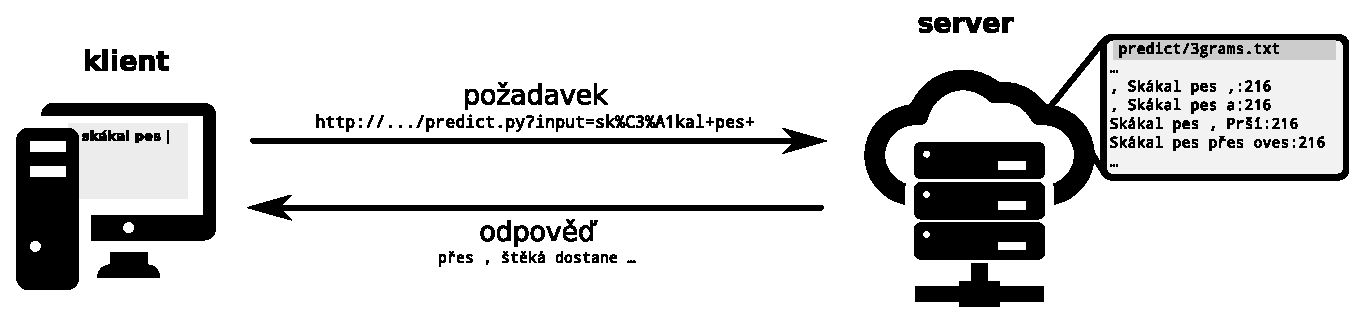
\includegraphics[width=1.0\textwidth]{client-server-schema1.eps}
	\caption{Schéma komunikace klienta a~serveru\protect\footnotemark}
	\label{fig:clientserver}
\end{figure}

\footnotetext{Schéma obsahuje ikony od Freepik vytvořené pod licencí Creative Commons BY 3.0}

\section{jQuery}

Knihovna jQuery\footnote{\url{https://jquery.com/}} je navržená pro usnadnění programovaní v~jazyce JavaScript. Zaměřuje se především na zjednodušení zpracování prvků v~HTML dokumentu, práci s~událostmi (např. stisk klávesy) a~komunikaci mezi klientem a~serverem pomocí Ajaxu.
% https://jquery.com/ 

\begin{spacing}{1.05}
\section{HTML}

HTML je standardní značkovací jazyk velice podobný jazyku XML. Je hojně používaný při tvorbě elektronických dokumentů pro webové prohlížeče, jako je kupříkladu Mozilla Firefox\footnote{\url{https://www.mozilla.org/en-US/firefox/desktop/}}. Webové prohlížeče jsou schopny HTML zpracovat a~zobrazit uživateli výslednou stránku, která obsahuje vizuální prvky a~textové formátování. \parencite[19--22]{raggett1999html}

Standard HTML vychází ze obecného značkovacího jazyka SGML (Standard Generalized Markup Language), který je založen na dvou principech, a~to že by značkovací jazyk měl být deklarativní, tedy popisovat strukturu a~další atributy, spíše než definovat způsob, jakým je dokument zpracováván, a~že by definice v~dokumentu měly být jednoznačné a~pevně definované, aby byl dokument zpracovatelný stejně jako například programový kód. \parencite{rubinsky1990sgml} %  cit. https://en.wikipedia.org/wiki/Standard_Generalized_Markup_Language --vytahat primarni zdroje, budou-li 


HTML popisuje strukturu stránky po sémantické stránce a definuje (částečně či úplně) její vzhled. Rozdíl mezi sémantickou informací a~informací o~tom, jak by měla prezentace vypadat, lze ilustrovat na dvojici značek, jejichž výsledná prezentace je zpravidla identická, a~to {\tt <strong>} a~{\tt <b>}. Značka {\tt <strong>} webovému prohlížeči říká, že text uvnitř této značky je důležitější než okolní text a~měl by podle toho také být naformátován (tedy zpravidla tučným řezem písma), zatímco značka {\tt <b>} pouze indikuje, že by text v~ní uzavřený měl být naformátován tučně. %  cit. https://en.wikipedia.org/wiki/HTML --primarni zdroje?? 


Zde popisovaná aplikace využívá HTML relativně málo, protože se jedná o~zásuvný modul, který ze své podstaty nesmí ovlivňovat vzhled stránky, do níž si uživatel vloží CKEditor s~tímto modulem. V~rámci editačního pole se však vyskytla potřeba HTML použít pro zobrazení nabídky s~výběrem jednotlivých možných doplnění, z~nichž si uživatel může vybrat. Jakkoliv je tedy co do množství kódu HTML zastoupeno nejmenší částí ze zde popisovaných technologií, je jeho použití důležité pro komfort koncového uživatele.

\section{CSS}

Druhou technologií, která je relativně málo využita, ale pro koncového uživatele je zásadní z~hlediska uživatelské přívětivosti rozhraní, jsou kaskádové styly. Ty jsou také jednou ze základních technologií používaných pro webové prezentace a~zajišťují definice vizuálního vzhledu stránek napsaných ve značkovacím jazyce. \parencite{meyer2004cascading}

Hlavním smyslem CSS je oddělení obsahu webové stránky od její vizuální prezentace. To je důležité především pro snazší udržování stránky a~větší flexibilitu. Použití CSS navíc umožňuje zobrazit jednu stránku různými způsoby, jedním z~nichž může být například možnost zobrazení pro barvoslepé uživatele.

Ve zde popisované aplikaci je tedy CSS využíváno k~definici vizuální prezentace nabídky doplnění.
\end{spacing}

\chapter{Implementace}

\begin{figure}[h]
	\centering
	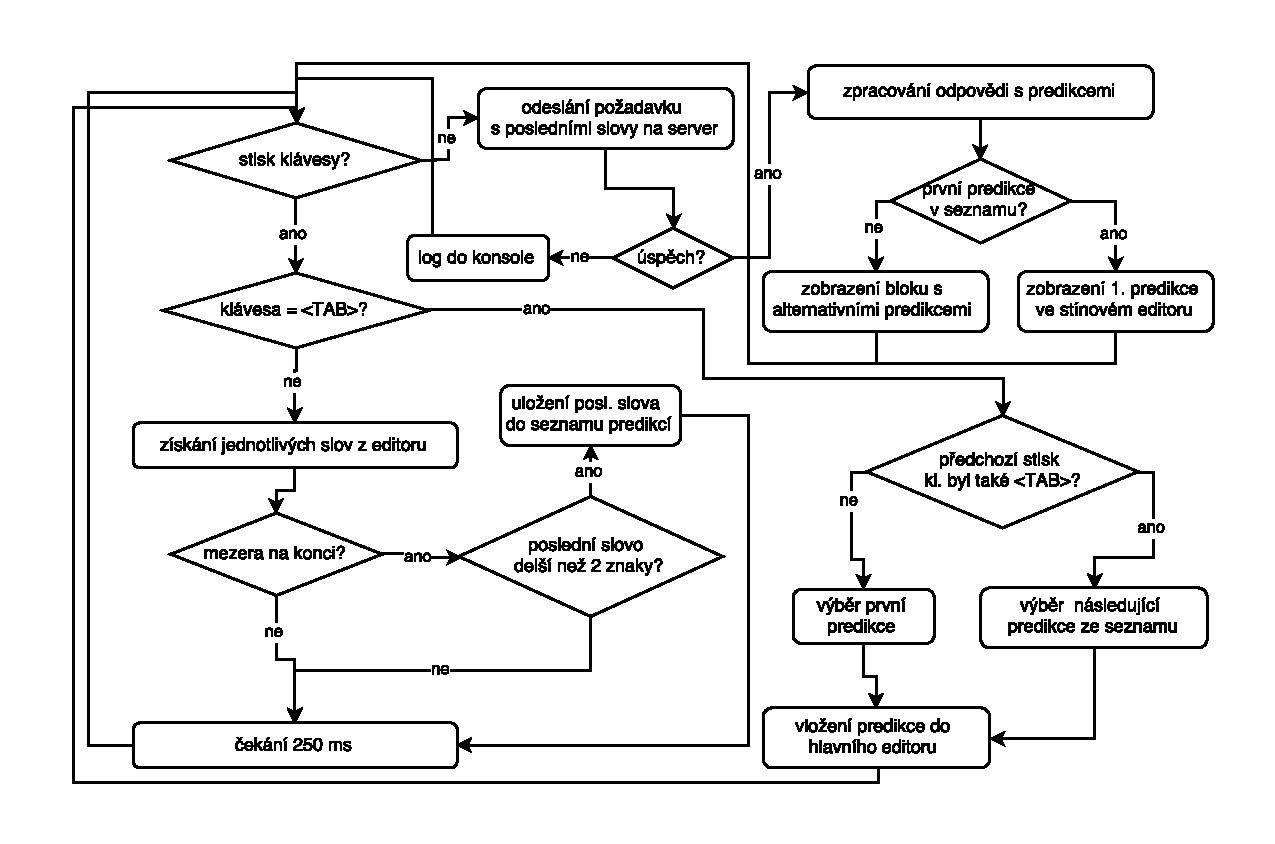
\includegraphics[width=1.0\textwidth]{autocomplete_floatchart.eps}
	\caption{Vývojový diagram pluginu}
	\label{fig:autocomplete_floatchart}
\end{figure}

\section{Uživatelské rozhraní}\label{ui}

Mluvit o~uživatelském rozhraní jako celku je v~tomto případě poněkud problematické, protože jde o~zásuvný modul a~není tudíž možné předvídat, jak přesně bude koncový uživatel modulu mít CKEditor nakonfigurován. V~této práci však postačí uvažovat základní konfiguraci CKEditoru tak, jak je poskytována na oficiálních webových stránkách\footnote{\url{http://ckeditor.com/}}. Tam jsou ke stažení tři předpřipravené balíčky, jež se liší množstvím zásuvných modulů, které jsou obsahují. Pro účely vývoje zde popisovaného pluginu i~pro účely samotného popisu byl vybrán nejmenší balíček {\it Basic Package}, který obsahuje 17 zásuvných modulů obstarávajících základní funkcionalitu. V~popisu práce s~editorem pak bude uvažována webová stránka, na níž se bude nacházet pouze CKEditor v~konfiguraci {\it Basic Package} s~přidaným pluginem, který je předmětem této práce.

Práce v~takto nakonfigurovaném editoru probíhá tak, že uživatel zadává text do editoru pomocí klasické klávesnice a~vybírá (případně nevybírá) si doplnění, která jsou mu nabízena. Doplnění jsou nabízena vždy, když uživatel na určitou dobu přestane vyvíjet aktivitu (pro účely testování se jako vhodné ukázalo být 250 ms). Aktivitou se myslí události {\tt keydown} a~{\tt keyup}, které reprezentují stisky kláves -- konkrétně stisknutí klávesy ({\tt keydown}) a~její uvolnění ({\tt keyup}). Nabídka se také nezobrazuje, když pro danou kombinaci slov a~písmen před pozicí kursoru nejsou nalezena doplnění. Ve chvíli, kdy si uživatel některé doplnění z~nabídky vybere, skript jej v~závislosti na situaci vhodným způsobem doplní do editoru a~posune na její místo kursor. Pokud uživatel za doplněné slovo vloží mezeru a poté nevyvine žádnou další aktivitu po 250 ms, zobrazí se mu další doplnění zvolené na základě předchozího slova zadaného (či vybraného) slova. V~ideálním případě by tak mělo na základě prvního slova být možné doplnit určité standardní věty pouhým vybíráním vhodných predikcí. Tomu ovšem zabraňuje nastavení aplikace, které filtruje z~nabídky predikcí příliš krátká slova (méně než tři znaky), protože ta většinou bývá rychlejší napsat celá manuálně.

\section{Zpracování textu v~editoru}

Aby mohla být serverovému skriptu odeslána data, na jejichž základě budou vyhledána možná doplnění, musí být na straně klienta zpracován text, který uživatel napsal do editoru. To probíhá v~několika krocích, jejichž výsledkem je řetězec předem definovaného počtu posledních slov v~editoru, který je vhodný k~odeslání na server.

Všechny operace spojené s~modifikacemi textu v~editoru i~prezentací nabídky predikcí jsou prováděny pouze v~případě aktivity uživatele. 

Prvním krokem je rozdělení obsahu editoru na jednotlivá slova. To zajišťuje funkce {\tt sliceContent()}, jež přijímá text editoru ve formě řetězce. Text rozděluje postupně na řádky podle tagu {\tt <br>}, kterým končí v~CKEditoru každý řádek, a~dále zpracovává pouze poslední řádek. To znemožňuje používat predikci na jiném než posledním řádku, což ale nevadí, protože momentálně plugin nepodporuje práci s~predikcemi na jiných místech než na úplném konci vkládaného textu. To je jeden ze známých nedostatků, který bude rozebrán v kapitole \ref{vyhodnoceni}. 

Následně funkce odstraní tagy HTML, nahradí nedělitelné mezery normálními a~rozdělí zpracovávaný řádek na jednotlivá slova. Jako datový typ pro uložení řetězce rozděleného na slova bylo zvoleno pole (array), jež má v~jazyce JavaScript připraveno velké množství metod vhodných pro tuto aplikaci. 

Jakmile má skript k~dispozici slova z~aktuálního (posledního) řádku v~editoru, se v~případě, že současné slovo u~kurzoru má délku alespoň tři znaky, zjišťuje pomocí funkce {\tt findLastSimiliarWord()}, zda se v~editoru už nevyskytuje slovo, které začíná na řetězec shodný se současným slovem a~má délku alespoň pět znaků. Pokud ano, přidá se do seznamu predikcí, který později bude uživateli nabídnut. Tento krok se provádí proto, že lze předpokládat, že pokud uživatel napsal jednou nějaké delší slovo a~znova začal psát slovo, které začíná stejnými znaky, bude chtít napsat téže slovo. Jde o~funkcionalitu podobou té z~textového procesoru LibreOffice Writer (obrázek \ref{fig:LOpredict}).

Po tomto kroku funkce {\tt getSuggestions()} provádí ajaxové volání na server za účelem získání predikcí vytvořených z~korpusových dat. Tato funkce přijímá několik hodnot, a~to pole se slovy z~posledního řádku, počet slov, která mají být odeslána na server, a~dále callback na funkci {\tt handleSuggestion()}, která zpracovává získaná doplnění.

Ve funkci {\tt getSuggestions()} proběhne připravení řetězce se slovy, která mají být odeslána na server. To znamená, že funkce metodou {\tt slice()} vyřízne z~pole posledních $N$ slov, kde $N$ je počet slov odesílaných na server a~výsledné pole $N$ prvků spojí do řetězce s~tím, že mezi jednotlivé prvky (slova) vloží znak {\tt +} (plus). Znak {\tt +} byl zvolen proto, že slova jsou odesílána, jak již bylo popsáno v~kapitole \ref{navrh}, metodou GET, tedy jako parametry adresy URL. V rámci dat odesílaných metodou GET lze reprezentovat mezeru buď znakem {\tt +} nebo řetězcem {\tt \%20}, přičemž tyto způsoby jsou v~praxi rovnocenné.

Následně funkce čeká předem nastavenou dobu (250 ms), zda nenastane další aktivita uživatele, a~v případě, že nenastane, odešle ajaxový požadavek na server.

V případě, že ajaxové volání na server uspělo (návratový kód {\tt 202 Success}), zavolá se pomocí callbacku, který byl funkci {\tt getSuggestions()} předán dříve, funkce {\tt handleSuggestion()}. Pokud volání z~jakéhokoliv důvodu skončilo chybou (kupříkladu nedostupnost server způsobí, že volání skončí návratovým kódem {\tt 404 Not Found}), vypíše se chyba do konzole a~z~pohledu uživatele se nic nestane. 

Funkce {\tt handleSuggestion()} přijímá jako argumenty mj. současné slovo pod kursorem, jeho případné doplnění z~existujícího textu v~editoru a~odpověď serveru. Odpověď serveru je řetězec znaků, který obsahuje slova oddělená od sebe znakem mezery. Funkce odpověď rozdělí na jednotlivá slova a~vyřadí slova kratší než 3~znaky včetně (z důvodů uvedených v~kapitole \ref{ui}). Pokud byla dříve nalezena predikce z~textu, je doplněním ze serveru předřazena, aby uživateli byla prezentována jako první. Poté jsou predikce nabídnuty uživateli.

\section{Zobrazení predikcí}

Nabídka predikcí sestává ze dvou různých částí. První z~nich je predikce (jíž může být celé slovo po mezeře, či část slova doplňující část již zadanou v~editoru), která se zobrazuje méně výrazně (šedě) ihned za zadávaným textem v~hlavním editoru (obrázek \ref{fig:nlp-predict}). Takové doplnění lze přijmout pouhým stiskem tabulátoru. Tento způsob zobrazení doplnění je inspirován řešením zobrazování automatického doplňování ve vyhledávači Google, které funguje na podobném principu. 

Pro toto řešení je využíváno tzv. stínového editoru, který je pomocí CSS umístěn přesně pod hlavní editor, v~němž uživatel zadává text. Do něj se pomocí JavaScriptové funkce {\tt copyContent()} ve zde popisovaném zásuvném modulu kopíruje text z~hlavního editoru. Pro zobrazení predikce je pak využíváno toho, že text zkopírovaný z~hlavního editoru má ve stínovém editoru identické prostorové vlastnosti jako text hlavního editoru a~na jeho konec lze snadno připojit aktuální predikci, která se tak zobrazuje uživateli fontem stínového editoru (ve zde popisované implementaci má stínový editor šedou barvu písma a~hlavní editor černou).

\begin{figure}[ht]
	\centering
	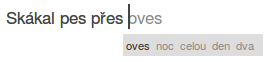
\includegraphics[width=0.4\textwidth]{nlp_predict_1}
	\caption{Zobrazení predikcí}
	\label{fig:nlp-predict}
\end{figure}

\subsection{Alternativní predikce}

Vzhledem k~tomu, že predikce nejsou vždy dokonalé nebo není možné jednoznačně rozhodnout, které slovo uživatel zamýšlí napsat, ukázalo se nutným zobrazovat i~alternativní predikce. 

Tyto alternativní predikce jsou prezentovány pod pozicí kursoru ve formě seznamu. Pokud chce uživatel využít některou predikci zobrazenou v~seznamu, stačí mu opětovně stisknout klávesu tabulátor, pomocí níž lze v~seznamu jednosměrně cyklovat mezi položkami. Aktuální položka se pak zároveň kopíruje do hlavního editoru, takže po dosažení požadované predikce uživatel vloží mezeru a~může pokračovat v~psaní. Tato metoda volby byla navržena především s~ohledem na původní cíl aplikace, tedy usnadnit psaní uživatelům, kteří z~mají z~nějakého důvodu problém zadávat text na klávesnici QWERTY. Cílem tedy není zrychlení psaní, jako tomu bývá u~implementací predikce textu například pro dotyková zařízení, ale co nejvíce snížit množství stisků různých kláves pro volby predikce.

Nabídka alternativních predikcí je zobrazována vždy pod kursorem, aby uživatel nebyl nucen dělit svou pozornost na různá místa obrazovky. O~zobrazení nabídky v~místě kursoru se stará funkce {\tt show\-Alternatives()}, která je závislá na funkci {\tt get\-Selection\-Coords()}. Z~pohledu problematiky implementace je zajímavá především funkce {\tt get\-Selection\-Coords()}, která pomocí zjišťování pozice aktuálního výběru\footnote{Více o výběrech v kapitole \ref{vybery}} textu získává absolutní pozici kursoru na obrazovce, jež je nutná pro správné zobrazení alternativ. Implementace výběrů se může lišit podle konkrétního prohlížeče, avšak obecně lze říci, že aktuální výběr vždy končí v~místě, kde je právě umístěn kursor. S~ohledem na tuto skutečnost a~na to, že API (application program interface) moderních prohlížečů umožňují získat pozice začátku a~konce výběru, lze pozici konce aktuálního výběru považovat za pozici kursoru, na níž se má zobrazit nabídka alternativních doplnění. 

\section{Vkládání predikcí}

Poté, co si uživatel vybere predikci tím, že stiskne klávesu tabulátor, zbývá ji vložit na správné místo, tedy na pozici kursoru.

V případě vkládání celého slova, nikoliv doplnění zbytku již zadaného slova, je vložení predikce relativně triviální. Jde pouze o~připojení dané predikce za pozici kursoru, přidání mezery a~přesun kursoru za ni. Jak bylo naznačeno výše, pokud se uživatel rozhodne cyklovat v~seznamu alternativních predikcí, vkládají se tyto do hlavního editoru automaticky pomocí funkce {\tt printCompletions()}. Chce-li uživatel využít první predikce, použije se při stisku klávesy tabulátor stejná funkce. 

V~případě doplňování pouhé části slova jde vzhledem k~tomu, že serverový skript ve všech případech vrací celá slova, o~úkon, který představuje zásah do již existujícího textu v~hlavním editoru. Pokud tedy uživatel napíše jako poslední slovo řetězec \exmp{p} a~předcházející slovo je \exmp{vážený}, navrácená slova jsou \exmp{paciente}, \exmp{pane}, etc. Je tedy zřejmé, že nelze zvolenou predikci vložit přímo za existující text, ale je nutné nějakým způsobem zabránit duplikaci částí slov. Tento problém je řešen ve funkci {\tt insertCompletion()} smazáním již napsané části slova z~predikce, jejíž zbytek je pak vložen za napsaný text. Do hlavního editoru se tedy nevkládá celá predikce \exmp{paciente}, nýbrž pouze její zbývající část po odtržení již napsané části, tedy například \exmp{aciente}.

Úplně poslední úkon, který se provádí, je přesunutí kursoru na korektní pozici poté, co byla predikce vložena do hlavního editoru. Je evidentní, že kursor nemůže zůstat na původním místě, na němž byl před vložením predikce, protože pak by uživatel buď psal další text před vloženou predikci, nebo by musel manuálně přejít na konec vkládaného textu. 

\subsubsection{Výběry}\label{vybery}

Manipulace s~kursorem v~textu se v~prohlížečích provádí pomocí výběrů. Výběr je objekt, který reprezentuje text označený v~textovém poli, přičemž může mít i~nulovou délku v případě, že není označen žádný text. Výběr má různé vlastnosti včetně pozice, s~nimiž lze manipulovat \parencite{mdn2015selections}. Pozice výběru může být vyjádřena dvěma způsoby, a to jako absolutní pozicí na obrazovce, tedy pixelovými souřadnicemi, nebo jako pozice v~textu, tedy počet znaků relativní k určitému místu v textu. % https://developer.mozilla.org/en-US/docs/Web/API/Selection

Přesun kursoru je tedy řešitelný přemístěním výběru v~textu o~délku predikce dále, ale v~praxi se ukazuje, že existuje nezanedbatelné množství případů, kdy zjišťování pozice výběru v~textu není přesné, a~tudíž výsledná pozice kursoru nemusí být správná. Z~toho pramení i~nedokonalosti v~implementaci popsané v~kapitole \ref{vyhodnoceni}.

\chapter{Vyhodnocení}\label{vyhodnoceni}

Z~testování během vývoje zásuvného modulu, který je předmětem této práce, lze potvrdit, že jeho použití šetří počet úhozů nutný k~napsání textu, takže cíl práce byl splněn. Vzhledem k~tomu, že se zásuvný modul zatím nedočkal nasazení v~reálných situacích, nelze jeho skutečný přínos uživatelům hodnotit.

Množství ušetřených úhozů značně závisí na povaze textu, který uživatel píše. V~rámci vývoje bylo provedeno krátké manuální testování na odlišných textech, které ukázalo, že kvalita predikcí je velmi závislá na podobnosti zdrojového korpusu a~psaného textu. Vzhledem k~tomu, že při testování byly použity n-gramy z~korpusu czTenTen12, nejlepších výsledků dosahoval systém na textech ze zpravodajských serverů, kde bylo dosaženo KSPC cca 0,4. Naopak v~případě, že text obsahoval například osobní jména, byla účinnost predikce výrazně omezena. Nejhoršího výsledku bylo dosaženo na textu mírně technického rázu (manuál k instalaci počítačového programu), a~to KSPC cca 0,7. Do úhozů byly počítány všechny klávesy.

Nutno podotknout, že se v~predikcích mnohdy vyskytovalo správné slovo, ale bylo ve špatném tvaru. Je tedy zřejmé, že by predikci značně vylepšila syntaktická analýza, případně kdyby doplňování probíhalo po částech, tedy nejdříve kmen slova a~poté jeho koncovka.

Další problémy, které potenciální uživatel zaznamená, jsou technické nedostatky frontendu. Hlavním z~nich je ten, že implementace momentálně neumožňuje práci vprostřed těla textu, ale pouze na jeho konci. Není tak možné mít text, do jehož části chce uživatel napsat odstavec s~využitím predikce. Zde je tedy značný prostor pro zlepšení.

Technicky příbuzný problém je pak omezená podpora formátovaného textu. Umístění predikcí a~pozice kursoru mohou být při výskytu formátovaného textu v~editoru nepřesné. To je vzhledem k~faktu, že CKEditor je editor typu WYSIWYG, další limitace, kterou je před reálným nasazením nutno vyřešit.

Celkově ale je implementace frontendu pro psaní s~výrazně sníženým průměrným množstvím úhozů na znak použitelná již nyní.

\clearpage

\chapter*{Závěr}

\addcontentsline{toc}{chapter}{Závěr}

Byla vyvinuta aplikace, která umožňuje zadávání textu bez nutnosti stisku všech kláves korespondujících s~písmeny ve slovech zadávaného textu. Pokud uživatel chce zadat text, jehož slova existují v~korpusu, z~něhož jsou vybírány predikce, má možnost z~těchto predikcí vybrat vhodně ty, které odpovídají jeho záměru, a~snížit tak počet úhozů na znak na hodnotu menší než jedna. Vzhledem k~velikosti korpusu, z~něhož jsou predikce vybírány, je rozumné předkládat, že takového výsledku lze dosáhnout téměř s~libovolným textem v~českém jazyce, což prokázaly i krátké testy. Současná implementace navíc umožňuje snížit počet stisknutých kláves na počet znaků v~textu také tím, že mezi predikce zařazuje již zadaná delší slova. Tato funkcionalita může být užitečná například pro uživatele, kteří zadávají text s~větším množstvím dlouhých odborných termínů (dobrým příkladem budiž lékařské texty).

V dalším vývoji by bylo vhodné zaměřit se především na problém s~tvary slov, jehož řešením může být buď syntaktická analýza nebo nabízení predikcí po částech, tedy oddělit kmen a~koncovku. Tímto krokem by bylo možné dále snížit hodnotu KSPC a~navíc by se tím eliminoval problém frustrace uživatele, který, vidí-li požadované slovo ve špatném tvaru, musí přemýšlet, zda je výhodnější predikci v~chybném tvaru zvolit a~opravit koncovku, nebo celé slovo napsat bez využití predikce. 

\clearpage

\pagestyle{plain}

% \begin{spacing}{0.7}
\printbibliography[title={Seznam literatury}]
% \end{spacing}

\addcontentsline{toc}{chapter}{Seznam literatury}

\end{document}
